\immediate\write18{makeindex -s nomencl.ist -o Outputs/rapport.nls Outputs/rapport.nlo}

\documentclass[11pt]{article}

%Langue et encodage :
 \usepackage[T1]{fontenc}
 \usepackage[utf8]{inputenc}
 \usepackage{lmodern}
 \usepackage[french]{babel} \usepackage{lmodern}


%Mise en page
\usepackage[a4paper, margin=2.5cm]{geometry}	%Papier
\usepackage{arev}									%Police
\renewcommand{\baselinestretch}{1.15} 				%Interligne
\setlength\parindent{4pt}							%Alineas
\usepackage[skip=5pt,font=footnotesize]{caption}
\usepackage{float}
\usepackage{xcolor}									%Couleurs perso
\definecolor{grisPerso}{rgb}{0.9,0.9,0.9}
\usepackage{tabu}

%Contenu :
\usepackage{hyperref}								%Liens
\usepackage{amsmath}								%Math
\usepackage{listings}								%Code source
\lstset{
language=bash,
backgroundcolor=\color{grisPerso},
basicstyle=\footnotesize,
frame=single}
\usepackage[refpage]{nomencl}						%Nomenclature
\usepackage{xpatch}
\makenomenclature

%Dessins et schémas
\usepackage{graphicx}
\usepackage{epstopdf}
\epstopdfsetup{outdir=./}
\usepackage{tikz}
\usepackage{includes/tikz-uml}
\usetikzlibrary{positioning,chains,fit,shapes,calc}
\newcommand{\illu}[3]{%
	\begin{figure}[ht!]
			  \centering
			  \includegraphics[scale=#3]{Graphics/#1}
			  \caption{#2}
			  \smallskip
	\end{figure}}

\newcommand*\emptyPage{\newpage\null\thispagestyle{empty}\newpage}
\begin{document}

\begin{titlepage}
\newgeometry{top=2cm,bottom=2cm}

\newcommand{\HRule}{\rule{\linewidth}{0.5mm}} % Defines a new command for the horizontal lines, change thickness here

\center % Center everything on the page
 
%----------------------------------------------------------------------------------------
%   HEADING SECTIONS
%----------------------------------------------------------------------------------------


\includegraphics[scale=0.6]{Graphics/logo.png}\\[1.5cm]

\textsc{\Large Projet Electif (technique)}\\[0.5cm] % Major heading such as course name
\textsc{\large Projet technique}\\[0.5cm] % Minor heading such as course title

{\normalsize \today}\\[1.5cm]

%----------------------------------------------------------------------------------------
%   TITLE SECTION
%----------------------------------------------------------------------------------------

\HRule \\[0.4cm]
{ \Large \bfseries Evolution de véhicules autonomes dans un environnement urbain intelligent}\\[0.4cm] % Title of your document
\HRule \\[2.5cm]


%----------------------------------------------------------------------------------------
%   LOGO SECTION
%----------------------------------------------------------------------------------------

 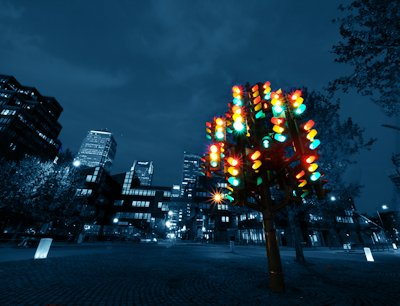
\includegraphics[scale=0.45]{Graphics/illustration.jpg}\\[2.5cm]

%----------------------------------------------------------------------------------------
%   AUTHOR SECTION
%----------------------------------------------------------------------------------------
{\normalsize Auteurs:}\\
\small
\textsc{Biton} Guillaume (guillaume.biton@ipsa.fr)\\
\textsc{Guichard} Marc-Antoine \small(marc-antoine.guichard@ipsa.fr)\\
\textsc{Lhermite} Camille \small(camille.lhermite@ipsa.fr)\\
\textsc{Monnot} Maxime \small(marc-antoine.guichard@ipsa.fr)\\[1cm]

 
%----------------------------------------------------------------------------------------

\vfill % Fill the rest of the page with whitespace

\restoregeometry

\end{titlepage}

\setcounter{secnumdepth}{5}
\setcounter{tocdepth}{5}

\newpage
\tableofcontents
\newpage
\pagenumbering{arabic}

\section*{Remerciements}

	Nous remercions Mesdames Assia Belbachir et Sorore Benabid, ensignants chercheurs au sein du laboratoire Mécatronique, Signal et Systèmes de l'IPSA pour nous avoir soumis cette idée, pour nous avoir accordé leur confiance quant à sa réalisation potentielle et pour leur soutien dans le cadre de ce projet.

	\vspace{80pt}

\section*{Notes préliminaires}
	L'ensemble des illustrations présentes dans ce dossier, sauf indication contraire dans leurs légendes, sont des réalisations personnelles et ne sont donc soumises à aucun droit particulier.\\

	Le travail de recherche ici présenté est sous la responsabilité des auteurs cités en première de couverture et sous la propriété de l'IPSA. Merci de nous contacter au moyen des adresses fournies pour nous signaler tout problème, ou pour toute demande liée à l'utilisation du contenu.\\

	L'ensemble des abréviations utilisées dans ces pages sont explicitées en page \pageref{nomenclature} (nomenclature).\\

	Les numéros entre crochets pouvant apparaitre au sein de paragraphes sont des références bibliographiques et vous renvoient à la page \pageref{bibliographie} (bibliographie).\\

	Ce dossier comprend de nombreuses références dynamiques, et pour un confort de lecture optimal, nous vous conseillons d'en lire la version numérique afin de pouvoir bénéficier des liens cliquables.\\

	Exception faite des modèles mécaniques en CAO 3D effectués sous Catia\textsuperscript{\textregistered}, l'ensemble des réalisations ici présentées utilisent des outils Open-Source : le présent dossier est rédigé en \href{https://www.latex-project.org/}{\LaTeX}, les illustrations ont été réalisées en dessin-vectoriel sous \href{https://inkscape.org/fr/}{Inkscape} ou en matriciel sous \href{https://www.gimp.org/}{GIMP} et les schémas et circuits électroniques sous \href{http://kicad-pcb.org/}{KiCad}.

\newpage

\section{Introduction}

	La voiture autonome, loin du concept de science-fiction qu'elle pouvait représenter il y a quelques années est en train de devenir une réalité.\\

Si cette ambition put être à une certaine époque motivée par le simple attrait de la prouesse technique, nous percevons aujourd'hui tous les bénéfices que l'on pourrait en tirer.
En effet, les avancées scientifiques et techniques nous permettent désormais de prétendre à concevoir une voiture qui soit non seulement autonome, mais surtout intelligente. Il est aujourd'hui tout à fait réaliste de penser que dans les quelques années à venir les voitures sauront adopter un comportement bien plus intelligent que celui de leurs conducteurs actuels, et ce au profit de la sécurité, de l' efficience énergétique mais également de l'encombrement des axes routiers.\\

A terme, nous pouvons facilement imaginer que les différents véhicules auront la possibilité de communiquer entre eux afin de prévenir les véhicules environnants de leurs intentions, mais cela ne les dispensera pas de devoir être capables d'évaluer leur environnement afin d'y détecter les éléments "indépendants" (piétons, obstacles...). \\

Comme toute révolution technologique, la voiture intelligente devra faire face au caractère progressif de son adoption: toutes les voitures sur les routes ne deviendront pas autonomes du jour au lendemain. Ces véhicules devront donc également être capables d'évoluer au milieu d'une circulation telle que nous la connaissons, où chaque acteur adopte un comportement presque parfaitement aléatoire, et ne signale pas toujours ces intentions.\\

Si les voitures deviennent intelligentes, c'est également le cas, depuis quelques années déjà, de la signalisation. Ainsi, de plus en plus de feux adaptent leur comportement au trafic, ce qui s'inscrit également dans une démarche d'optimisation de la circulation. Il est très réaliste d'espérer que cette technologie déjà existante se fera omniprésente dans les années qui viennent, d'où notre volonté d'inclure cet élément d’environnement à notre projet.\\

Le but de ce projet est donc d'étudier notre capacité à faire cohabiter intelligence artificielle et environnement "réel" et indépendant avec des moyens techniques et financiers extrêmement restreints, mais également et surtout de fournir une plateforme d'expérimentation aux étudiants de l'IPSA (et d'ailleurs ?) afin de faciliter l'apprentissage des sciences de la mécatronique et de l’intelligence artificielle tout en ancrant ce savoir dans une réalité pratique et stimulante.

\newpage
\section{Définition du besoin}

	Une définition pertinente du besoin est une condition absolument nécessaire pour la bonne réalisation de tout projet. Nous nous emploierons donc à définir aussi précisément et pertinemment que possible le besoin motivant ce projet, et à régulièrement revenir sur ce dernier afin de prendre en compte d'éventuelles évolutions et à prévenir toute dérive du projet.

\subsection{Besoin}
Le besoin à l'origine de ce projet fut exprimé par mesdames A. Belbachir et S. Benabid en tant qu'enseignants chercheurs au laboratoire Mécatronique, Signal et Systèmes à l'IPSA. Leur souhait était de bénéficier d'une plateforme articulée autour de robots autonomes évoluant dans une simulation d’environnement urbain, capables de détecter des feux de signalisation "intelligents" et d'adapter leur comportement en conséquence. Cette plateforme pourrait servir de support de TP\nomenclature{TP}{Travaux Pratiques} dans l'ensemble des matières enseignées par le département, mais également servir de "vitrine" voir même de plateforme de recherche.\\

Les principales fonctionnalités évoquées étant :
\begin{itemize}
	\item \textbf{La reconnaissance d'image} pour la détection des feux de signalisation.
	\item \textbf{La présence de feux bicolores commandés par FPGA\nomenclature{FPGA}{PGA (Field-Programmable Gate Array, ou Réseau de Portes Programmables : un type très répandu de circuit logiques programmables.}.} Ces feux seraient "intelligents" dans le sens où il s'adapteraient à la circulation. La présence de capteurs de présence est donc induite.
\end{itemize}

\subsection{Précision du besoin}

Ayant suivi nombre de matières enseignées par le département et participé à de nombreuses séances de travaux pratiques, nous bénéficions d'une image relativement claire des implications de ce projet ainsi que des contraintes relevant pour la plupart du simple bon sens.
Dans un soucis de clarté et d'application de "bonnes pratiques" nous prîmes cependant soin de valider l'ensemble de ces éléments au cours de réunions avec nos "clients" du laboratoire.\\

Ainsi, nous ajoutâmes les points suivants à la liste des exigences :
\begin{itemize}
	\item "Côté circuit" :
	\begin{itemize}
		\item \textbf{Le circuit devra bénéficier d'un encombrement raisonnable}.
		\item \textbf{Les feux de circulation devront pouvoir être commandés via une carte FPGA}.
	\end{itemize}
	\item "Côté robots" :
	\begin{itemize}
		\item \textbf{Les robots devront pouvoir être utilisés en classe sans que les préoccupations matérielles ne soient accaparantes}.
		\item \textbf{Les robots devront pouvoir être programmés en utilisant les langages enseignés à l'IPSA} à savoir C et C++ et ses variantes (Arduino...), Python, voir même Matlab...
		\item \textbf{Les robots devront bénéficier de possibilités d'application flexibles :} les enseignements étant ciblés, il est important que les utilisateurs des robots puissent se concentrer sur un aspect de leur utilisation sans avoir à se soucier des autres. De même, les robots devront embarquer suffisamment de capteurs ou tout du moins de capacité d'extensions pour que cela ne soit pas un facteur limitant lors de l'élaboration de sujets de TP.
		\item \textbf{Les robots devront ne pas pouvoir représenter un danger pour ses utilisateurs}.
	\end{itemize}
\end{itemize}
\newpage
\section{Étude du besoin}

	\subsection{Analyse du besoin}

Le besoin exprimé précédemment comporte un certain nombre d'implications logiques.
Leur prise en compte relève déjà du domaine de la solution, mais reste d'ordre suffisemment général pour être évoquée ici. Surtout, ces points seront à prendre en compte lors de l'élaboration d'une solution "détaillée".\\

Reprenons les points évoqués ci-avant:

\renewcommand{\labelitemi}{\textbullet}
\renewcommand{\labelitemii}{$\Rightarrow$}
\renewcommand{\labelitemiii}{-}
\renewcommand{\labelitemiv}{\textbullet}

	\subsubsection{Pour le circuit}
		\begin{itemize}
			\item \textbf{Le circuit devront bénéficier d'un encombrement raisonnable}.
			\begin{itemize}
				\item Les dimensions du circuit devront être raisonnables.
				\item Nous songerons également à une structure démontable (qui devra rester simple à assembler).
			\end{itemize}
			\item \textbf{Les feux de circulation devront pouvoir être commandés via une carte FPGA}.
			\begin{itemize}
				\item Une carte adaptant les tensions et courants et disposant de connecteurs adaptés aux caractéristiques des cartes possédées par l'IPSA devra être proposée.
			\end{itemize}
		\end{itemize}
	\subsubsection{Pour le robot}
		\begin{itemize}
			\item \textbf{Les robots devront pouvoir être utilisés en classe sans que les préoccupations matérielles ne soient accaparantes.}
			\begin{itemize}
				\item Cela implique plusieur points :
				\begin{itemize}
					\item Bénéficier d'une autonomie suffisante pour que l'ensemble des groupes puissent effectuer leurs manipulations au cours d'une séance entière sans que cela ne nécéssite de charger/remplacer la batterie. D'expérience, nous estimons l'autonomie minimum à une heure pour répondre à ce critère.
					\item Présenter des connecteurs et des interfaces permettant une intéraction "technique" avec le robot ne nécéssitant pas de matériel complexe. Ceci passe par une possibilité de changer ou recharger la batterie sans outils particuliers, de pouvoir programmer le robot via USB ou réseau plutot que via un port parallèle par exemple, ou encore proposer au minimum un bouton accessible permettant le lancement d'un séquence de code prédéfinie.
					\item Etre d'une conception suffisemment robuste pour pouvoir être manipulé quotidiennement sans en "souffir" et suffisemment simple pour pouvoir être aisément entretenu.
				\end{itemize} 
			\end{itemize}
			\item \textbf{Les robots devront pouvoir être programmés en utilisant les langages ensignés à l'IPSA.}
			\begin{itemize}
				\item Cette problématique sera étudiée plus en détail en \ref{Solution-controleur} (page \pageref{Solution-controleur})
			\end{itemize}
			\item \textbf{Les robots devront bénéficier de possibilités d'application flexibles.}
			\begin{itemize}
				\item Ceci passe par une \textbf{modularité totale} des différents éléments qui composent le robot, aussi bien sur le plan matériel que logiciel. Cette modularité devra rester une préoccupation de premier plan tout au long du développement de ce projet.
			\end{itemize}
			\item \textbf{Les robots devront ne pas représenter de danger pour ses utilisateurs}.
			\begin{itemize}
				\item La structure du robot ne devra pas présenter d'éléments tranchants.
				\item La partie élecctrique et électronique devra employer des puissances raisonnables, et être protégée contre les forts courants.
			\end{itemize}
		\end{itemize}


\subsection{Diagrammes des cas d'utilisation}

Toujours dans un soucis de clareté et de bonne pratiques, nous avons ébauché les diagrammes des cas d'utilisation de haut niveau suivants :

	\subsubsection{Pour le circuit :}

		\begin{tikzpicture} 
			\setcounter{tikzumlUseCaseNum}{0}
			\begin{umlsystem}[x=10, fill=blue!10]{Circuit} 
				\umlusecase[fill=white]{Brancher la carte FPGA} 
				\umlusecase[y=-2,fill=white]{Evoluer en autonomie} 
				\umlusecase[y=-4,fill=white]{Mettre en place le circuit}
				\umlusecase[y=-6,fill=white]{Ranger le circuit}  
			\end{umlsystem} 
			 
			\umlactor[y=0.5]{Développeur}  
			\umlactor[y=-2.5]{Utilisateur} 
			   
			\umlinherit{Développeur}{Utilisateur} 
			\umlassoc{Développeur}{usecase-1} 
			\umlassoc{Utilisateur}{usecase-2} 
			\umlassoc{Utilisateur}{usecase-3}  
			\umlassoc{Utilisateur}{usecase-4}  
		\end{tikzpicture}

	\subsubsection{Pour le robot :}

		\begin{tikzpicture} 
			\begin{umlsystem}[x=10, fill=blue!10]{Robot} 
			\umlusecase[fill=white]{Charger un programme} 
			\umlusecase[y=-2,fill=white]{Evoluer en autonomie} 
			\umlusecase[y=-4,fill=white]{Changer la batterie} 
			\end{umlsystem} 
			 
			\umlactor{Développeur}  
			\umlactor[y=-3]{Utilisateur} 
			   
			\umlinherit{Développeur}{Utilisateur} 
			\umlassoc{Développeur}{usecase-1} 
			\umlassoc{Utilisateur}{usecase-2} 
			\umlassoc{Utilisateur}{usecase-3}	 
		\end{tikzpicture} 

		\textbf{Reprogrammation :}
		\begin{itemize}
			\item \textbf{Précondition :} Nous disposons d'un programme fonctionnel.
			\item \textbf{Déclencheur :} Un développeur souhaite implémenter un programme.
			\item \textbf{Scenario :}
			\begin{enumerate}
				\item On connecte le robot à une source de tension.
				\item On établit une liaison entre le robot et un ordinateur.
				\item Le développeur lance le téléversement du programme.
				\item Le robot acquitte.
				\item On ferme la connexion.
			\end{enumerate}
		\end{itemize}

		\textbf{Evolution en autonomie:}
		\begin{itemize}
			\item \textbf{Précondition :} Le robot a été programmé et dispose d'une batterie chargée.
			\item \textbf{Déclencheur :} Un membre du laboratoire souhaite observer le comportement du robot.
			\item \textbf{Scenario :}
			\begin{enumerate}
				\item On met le robot sous tension.
				\item On place le robot sur une ligne blanche du circuit.
				\item On appuie sur le bouton de démarrage de séquence
				\item Le robot déclenche les programmes en mémoire.
			\end{enumerate}
		\end{itemize}

		\textbf{Changement de batterie:}
		\begin{itemize}
			\item \textbf{Déclencheur :} On souhaite changer la batterie du robot
			\item \textbf{Scenario :}
			\begin{enumerate}
				\item On met le robot hors tension.
				\item On accède à la batterie en place le cas échéant, et on la retire.
				\item On met en place la nouvelle batterie
				\item On remet en place les éléments éventuellement retirés pour accéder à la batterie.
			\end{enumerate}
		\end{itemize}


		Le mode d'utilisation primaire est bien évidemment celui de l'évolution en autonomie. Le robot étant destiné à servir de plateforme de recherche, et devant donc être entièrement reprogrammable, il est délicat de décrire ce mode d'utilisation qui dépendra intégralement du programme chargé par l'utilisateur.\\

		Nous nous appliquerons cependant à décrire le mode d'utilisation correspondant à l'application la plus basique du robot (et de fait au programme que nous livrerons avec ce dernier).

\newpage
\section{Élaboration d'une solution}

	\subsection{Circuit}


\subsection{Robot}

	\subsubsection{Suivi de trajectoire}

		Afin d’offrir une capacité de suivi de trajectoire simple et robuste, il a été décidé d’intégrer au robot la fonctionnalité "suivi de ligne". Il s’agit de l’une des méthodes les plus répandues\cite{bib3} \cite{bib4}, relativement simple à implémenter et économe aussi bien en composants qu’en puissance de calcul nécessaire.\\

		L’idée est d’offrir une base fiable et simple pour que le suivi de trajectoire ne soit pas une source de préoccupation ou d’erreur dans le cas d'utilisations centrées sur d’autres problématiques (dans le cadre d'un TP sur la reconnaissance d'image, par exemple). Cela n’exclut cependant pas qu’un étudiant ou chercheur désireux d’explorer d’autres possibilités de suivi de trajectoire (via la caméra, un dispositif de triangulation ou autre) puisse se passer de ce module et exploiter une autre solution.\\

		Le principe de suivi de ligne est relativement simple : on place sur l’axe du robot, quelques millimètres au-dessus du sol, un capteur appelé « réflecteur optique ». Ce capteur émet une onde lumineuse (souvent infrarouge) et une cellule mesure l’intensité reçue sur la longueur d’onde émise. Une forte intensité reçue indiquera la présence d’une surface réfléchissante, tandis qu’une faible intensité indiquera la présence d’une surface absorbante. Il est ainsi aisé de différencier un fond sombre (la « route ») d’une ligne blanche.\\

		Une loi linéaire lie la tension lue en sortie de capteur à l'intensité reçue.\\
		Une simple lecture de cette tension permet, après comparaison avec des valeurs "seuil" définies expérimentalement, de savoir si le capteur se trouve au dessus d'une ligne blanche ou non.\\

		Sur les schémas suivants, pour des raisons d'imprimabilité et de lisibilité, les lignes seront noires et le revêtement du circuit sera blanc.\\

		\begin{figure}[ht!]
			\centering
			\begin{minipage}{0.48\textwidth}
				\centering
				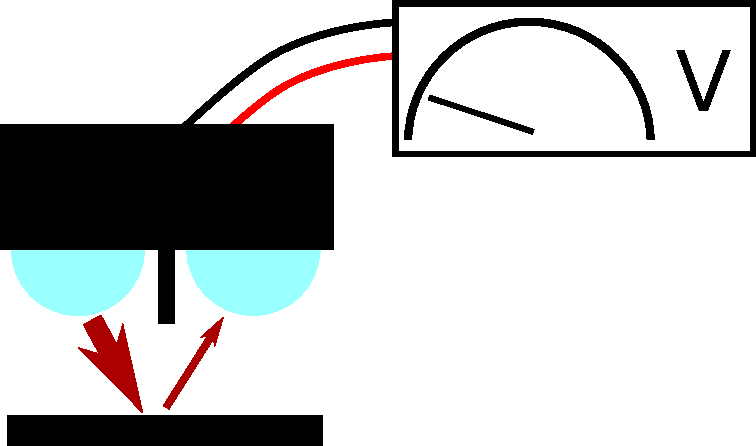
\includegraphics[scale=0.45]{Graphics/capteurOptiqueFondNoir.pdf}
				\caption{Capteur au dessus d'un support sombre}
			\end{minipage}\hfill
			\begin{minipage}{0.48\textwidth}
				\centering
				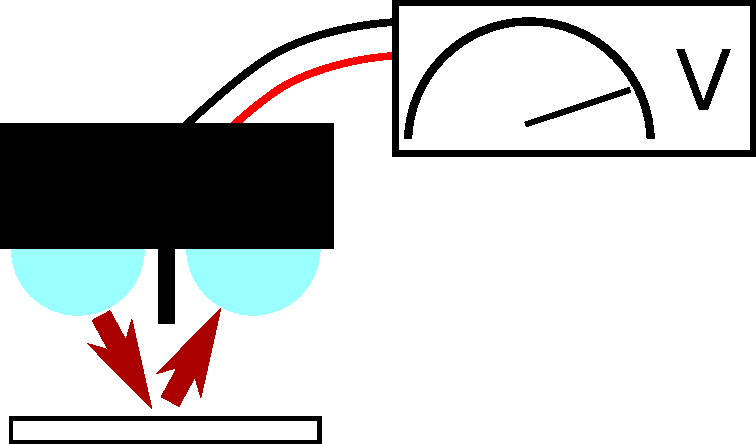
\includegraphics[scale=0.45]{Graphics/capteurOptiqueFondBlanc.pdf}
				\caption{Capteur au dessus d'un support clair}
			\end{minipage}
		\end{figure}

		La question qui se pose est celle du nombre de capteurs, et de leur disposition.\\

		Il est tout à fait possible de n'utiliser qu'un capteur : chaque fois qu'il quitte la ligne blanche, on entamera un virage à droite (puis à gauche si on ne retrouve pas la ligne blanche dans les quelques millisecondes suivantes) jusqu'à retrouver la ligne. Il est évident que cette méthode ne permettra pas une très grande fluidité de déplacement pour notre robot.

		\illu{capteurSimpleGauche.pdf}{Dépassement de la ligne sur la gauche}{1}
		\illu{capteurSimpleDroite.pdf}{Dépassement de la ligne sur la droite}{1}

		L'utilisation de deux capteurs permet une meilleure fluidité. On placera cette fois un capteur de chaque côté de la ligne.

		\illu{capteurDoubleGauche.pdf}{Dépassement de la ligne sur la gauche}{1.4}
		\illu{capteurDoubleDroit.pdf}{Dépassement de la ligne sur la droite}{1.4}

		Notons que, quelque soit la méthode employée, le suivi de ligne se résume toujours à un "rebondissement" des capteurs sur la ligne. Aussi, pour obtenir une trajectoire aussi rectiligne que possible, il faudra "resserer" les capteurs au maximum autour de la ligne, et appliquer des corrections de faible amplitude.

		\illu{capteurDoubleEcartFort.pdf}{Ecart important entre les capteurs}{1}
		\illu{capteurDoubleEcartFaible.pdf}{Ecart réduit entre les capteurs}{1}

		Nous pourrons éventuellement introduire un amortissement progressif de la correction via un régulateur PID\nomenclature{PID}{Proportionnel, Intégrateur, Dérivateur}, mais cela peut introduire de nombreuses problématiques dans des cas d'utilisation plus complexes.\\

		Nous retiendrons donc à ce stade la solution consistant en deux capteurs placés de part et d'autre de la ligne. Nous veillerons à ce que le placement des capteurs permette une détection de très faibles écarts de trajectoire, sans pour autant induire des ambiguïtés de mesure.\\

		Intéressons nous maintenant au cas d'une trajectoire courbe. Le fait d'avoir privilégié l'application de faibles corrections peut alors s'avérer problématique si ces dernières ne sont pas suffisantes pour adapter la trajectoire.

		\illu{perteTrajectoireVirage.pdf}{Perte de trajectoire en virage dû à de trop faibles corrections}{1.5}

		Pour obtenir un fluidité de déplacement raisonnable tout en assurant la possibilité de suivre des trajectoires courbes à rayon de virage réaliste, nous placerons une deuxième série de capteurs "encadrant" les capteurs principaux. Une détection de ligne par ces capteurs déclanchera une correction plus importante.

		\illu{trajectoireVirage.pdf}{Maîtrise de la trajectoire en virage grâce à l'utilisation de 4 capteurs}{1.5}

		Cette solution consistant en l'utilisation de quatre réflecteurs optiques alignés de manière à encadrer de près la ligne à suivre est sans doute l'une des plus simples imaginables en terme de réalisation mais également d'utilisation et de maintenance.
		Elle n'est malheureusement pas suffisante pour répondre à notre besoin. En effet, cette solution trouvera ses limites dès lors que notre Robot rencontrera sa première intersection, élément capital de ce projet.\\

		\illu{intersection4Capteurs.pdf}{Robot incapable de répondre à la présence d'une intersection}{1.5}

		Si on trouve dans la littérature de très nombreux exemples de réalisations de robots suiveurs de lignes, ces dernières se limitent toujours à des circuits sous forme de boucle. Notre défi est donc de mettre au point une solution permettant l'évolution du robot sur un circuit comprenant des intersections. Notre robot devra ne pas être "perturbé" au passage d'une intersection, mais surtout être capable d'emprunter toutes les directions qui lui sont offertes.\\

		La solution que nous avons mis au point consiste en l'introduction d'un capteur central et l'adoption d'un comportement "mono-latéralement centré" du robot lors de la traversée d'intersections : lorsqu'il arrivera sur une intersection, le robot ne se souciera plus que de garder son capteur central sur la ligne, et ses capteurs latéraux \textbf{du côté de la direction choisie} à l'écart de cette dernière.

		\illu{intersection5CapteursTD.pdf}{Suivi de trajectoire sur une intersection (en choisissant d'aller tout droit)}{1.5}
		\illu{intersection5CapteursDroite.pdf}{Suivi de trajectoire sur une intersection (en choisissant d'aller à droite)}{1.5}

		Notons que la forme de la ligne devra être intelligemment faite, en présentant des rayons de courbure réalistes (un véhicule ne peut pas tourner à angle droit) et des intersections réalisables (notamment via l'utilisation de deux lignes séparées pour la circulation en sens contraires).\\

		Voici donc à quoi ressemblerait un carrefour:
		\illu{carrefour.pdf}{Carrefour en représentation "lignes"}{1.4}

		Pour pleinement définir la logique mise au point, illustrons la au travers de la situation la plus complexe que pourra rencontrer notre robot, qui est celle de la bifurcation à gauche.

		\illu{carrefour5capteursGauche.pdf}{Cas du virage à gauche sur un carrefour avec cinq capteurs}{1.5}

		\begin{enumerate}
			\item Le premier croisement ne nous intéresse pas. Nous allons continuer tout droit et éteignons donc la moitié droite de nos capteurs.
			\item Au passage du croisement, nous éteignons temporairement l'ensemble de nos capteurs.
			\item Le croisement passé, nous éteignons cette fois la moitié gauche de nos capteurs pour ne pas être perturbés par "la voie d'insertion".
			\item Peu de temps après, nous rallumons la moitié gauche et éteignons la moitié droite des capteurs pour suivre la voie bifurquant à gauche.
		\end{enumerate}

		Cette solution semble robuste tout en conservant une certaine simplicité d’implémentation. Elle sous-entend en revanche que le robot "sache" quand il arrive sur une intersection, mais également qu'il puisse évaluer à quelques millimètres près la distance qui le sépare des différentes "parties" de cette intersection (pour activer et désactiver ses capteurs en conséquence).\\

		La solution à cette problématique nous a été inspirée par le souvenir d'un brevet déposé en 2003 par le groupe PSA \cite{bib5}, qui proposait l'utilisation de code-barres tracés sur la route et que des capteurs placés sous le pare-choc des voitures pourraient "lire" pour prévenir le conducteur des sources de danger à venir (intersections, feux...).
		Il fut donc décidé que deux capteurs supplémentaires seraient ajoutés sur les extérieurs. Ils augmenteraient ainsi la précision de placement sur la ligne, mais permettraient surtout de lire des "codes-barres" placés sur la piste. Ces code-barres devraient permettre au robot d'être averti de l'approche d'un carrefour (trois choix de direction possibles) ou d'une simple intersection (deux choix possibles). Nous avons simplement basé notre code sur une ligne simple ou doublée :\\
		\begin{figure}[H]
			\begin{tabu}to \textwidth {@{} | l | *3{X[c]|}@{}}
			  \hline
			   & \textbf{Gauche} & \textbf{Droite} & \textbf{Gauche ET Droite} \\
			  \hline
			  \textbf{Simple} & Impossible de tourner à droite & Impossible de tourner à gauche & Toutes possibilités offertes\\
			  \hline
			  \textbf{Double} & Obligation de tourner à gauche & Obligation de tourner à droite & Impossible d'aller tout droit \\
			  \hline
			\end{tabu}
			\caption{Formalisme employé pour les code-barres}
		\end{figure}

		Un code "doublé" serait composé de deux lignes elles mêmes séparées d'une épaisseur de ligne.
		Les codes seraient placés à 30cm du premier croisement.\\

		Dès la lecture d'un code au sol, le robot sera donc "attentif" à l'éventuelle apparition d'un doublon pendant environ deux centimètres. Si rien n'est lu passé cette distance, il en déduira qu'il s'agit d'un code simple. Il prendra alors une décision de direction (et pourra au passage en avertir les autres robots) et commencera un décompte de distance afin de gérer les activations et désactivations de ses capteurs jusqu'au franchissement de l'intersection.\\


		Illustrons ce système avec le cas de la bifurcation à gauche :

		\illu{carrefour7capteursGauche.pdf}{Cas du virage à gauche sur un carrefour avec sept capteurs}{1.5}

		\begin{enumerate}
			\item Lecture d'un code-barre : dans 30cm le robot aura la possibilité de tourner à droite et à gauche.
			\item Aucun doublon détecté dans les quelques centimètres suivants. La possibilité d'aller tout droit nous est donc offerte. Prise de décision quant à la direction (nous choisissons d'aller à gauche) et avertissement des autres robots en conséquence.
			\item Le premier croisement ne nous intéresse pas. Nous allons continuer tout droit et éteignons donc la moitié droite de nos capteurs.
			\item Au passage du croisement, nous éteignons temporairement l'ensemble de nos capteurs.
			\item Le croisement passé, nous éteignons cette fois la moitié gauche de nos capteurs pour ne pas être perturbés par "la voie d'insertion".
			\item Peu de temps après, nous rallumons la moitié gauche et éteignons la moitié droite des capteurs pour suivre la voie bifurquant à gauche.
		\end{enumerate}

		Le robot doit donc être conscient des distances parcourues avec une précision supérieure à deux centimètres. Le moyen le plus simple d'implémenter cette fonctionnalité est sans aucun doute au travers d'un encodeur incrémental placé sur l'axe de propulsion du robot.\\

		Nous pouvons donc considérer qu'à ce stade, nous disposons d'un solution satisfaisante répondant à la problématique du suivi de trajectoire.
		Cette solution répond précisément aux contraintes du projet, tout en conservant un certain niveau de simplicité. Elle est, pour rappel, constituée des éléments suivants :\\

		\begin{itemize}
			\item \textbf{Sur le circuit :} Un réseau de lignes blanches sur fond noir représentant les trajectoires empruntables par le robot.
			\item \textbf{Sur le robot :} Un ensemble de 7 réflecteurs optiques.
		\end{itemize}

	\subsubsection{Détection d'obstacles et de de signalisation}


	\subsubsection{Implémentation matérielle}

		\paragraph{Propulsion et direction}

			La solution la plus répandue en "petite robotique" consiste en l'utilisation de deux moteurs à courant continu pilotés indépendamment assurant à la fois la propulsion et la direction : on réduira les gaz à droite pour tourner de ce côté et réciproquement. Ces moteurs sont généralement pilotés en "PWM" \nomenclature{PWM}{Pulse-Width Modulation, ou Modulation de Largeur d'Impulsions}, mais d'autres solutions sont possibles et dépendront de notre contrôleur. Beaucoup d'applications utilisent des chenilles ou des courroies en caoutchouc pour assurer la propulsion, mais nous privilégierons l’utilisation de roues à pneus, par soucis de simplification de la conception (l'emploi de chenilles ou de courroies induit  une grande précision d'usinage et de montage pour assurer le parallélisme des poulies et la tension de la courroie) et de réduction des coûts.\\

			L'utilisation d'un seul moteur de propulsion et d'une roue directionnelle pilotée par un servomoteur a longtemps été considérée, mais cette solution s'est révélée bien plus complexe à mettre en place et sans réel intérêt particulier.\\

			\illu{virageDeuxMoteurs.pdf}{Virage à l'aide de deux moteurs indépendants}{1.5}

			L'espacement entre les deux roues $E$ est constant et connu.
			On fixera la vitesse appliquée à la roue à l'extérieur du virage $\omega_{ext}$ comme référence.
			On adaptera donc la vitesse de la roue à l'intérieur du virage $\omega_{int}$ en fonction du rayon de virage $R$ désiré.
			Il s'agit là d'une simple relation de Thales et on définit ainsi :
			\[\omega_{int} = \omega_{ext}\frac{R-E}{R}\]

			On peut donc obtenir n'importe quel rayon de virage en diminuant simplement la vitesse de la roue à l'intérieur du virage.
			L'approximation selon laquelle la tension appliquée à un moteur et sa vitesse de rotation sont linéairement liés sera amplement suffisante dans le cadre de ce projet.\\

		\paragraph{Controleur}\label{Solution-controleur}

			Nous cherchons un contrôleur capable d'embarquer des applications en C (ou ses dérivés) et si possible en Python et/ou Matlab.
			Ce contrôleur devra être capable d'acquérir les données de différents capteurs et de commander deux moteurs au minimum (sans compter d'éventuelles sorties type LEDs).
			Le contrôleur devra également bénéficier d'une puissance de calcul suffisante pour les opérations de reconnaissance d'image.\\

			Ce dernier critère élimine d'office les microcontrôleurs 8 et 16 bits et donc les cartes de type "Arduino" dont la puissance de calcul et la capacité de traitement de flux est bien trop faible pour permettre une reconnaissance d'image supérieure à quelques pixels carrés.\\

			Nous nous sommes naturellement tournés vers la famille des micro-ordinateurs mono cartes. Cette récente catégorie d'ordinateurs propose sur une carte de quelques centimètres de côté et pour moins d'une centaine d'euros un véritable ordinateur avec une connectivité réseau et USB, bien souvent vidéo, une puissance de calcul extrêmement confortable et la capacité de faire tourner des systèmes Linux et dérivés (et donc d’exécuter tous types de codes). Démocratisés en 2011 avec le Raspberry-Pi, ces ordinateurs se sont multipliés et l'offre est aujourd'hui très large. Nous avons ciblé notre sélection sur les plus rependus (qui sont, de par leur succès, bien plus abordables et faciles à se procurer, et bénéficient d'une plus large et solide base documentaire) : les Raspberry-Pis, Beaglebones et UDOOs (pour ne citer qu'eux).\\

			Les UDOOs furent vite écartés en raison de leur prix.
			Le Raspberry-Pi 2 et BeagleBone Green se situent dans la même gamme de prix (autour de 40\$). Nous avons arrêté notre choix sur le BeagleBone Green (BBG\nomenclature{BBG}{BeagleBone Green}): ce dernier, contrairement au Raspberry-Pi 2, ne dispose pas de sortie vidéo (dont nous n'avons pas utilité au sein de ce projet) et possède une puissance de calcul légèrement inférieur à ce dernier (tout en restant parfaitement respectable) mais possède une mémoire intégrée (ce qui dispense de l'achat d'une carte séparée) et surtout de capacités d'entrées/sorties numériques et analogiques bien supérieures. Ce point nous est extrêmement important: en effet, le Raspberry-Pi n'est capable de générer qu'un signal PWM et ne possède aucune entrée analogique ce qui aurait nécessité l'utilisation de "périphériques" supplémentaires pour la gestion des moteurs et des capteur et donc alourdi les coûts et la complexité de conception, augmenté le nombre de sources potentielles de pannes...\\

			Nous utiliserons donc un BeagleBone-Green Wireless :
			\illu{BBG.jpg}{Le BeagleBone Green \textit{\textbf{(source : seeedstudio.com)}}}{0.45}

			Ce dernier est équipé d'un processeur ARM 32bits à 1Ghz, de 512Mo de RAM de 4Go de mémoire embarquée et d'un impressionnante capacité de communication : 7 entrées analogiques (la carte comprend un convertisseur analogique-numérique 12bits), 65 entrées/sorties numériques (0 ou 3.3V) et bénéficie même de fonctionnalités telles qu'un compteur d'impulsion intégré au processeur (particulièrement utile pour l'interfaçage de notre encodeur). La connectivité wifi et bluetooth offre de belles possibilités quant aux interfaces utilisateur et la capacité de communiquer entre robots. La carte consomme moins de 1,5W et coûte 45\$ \cite{bib6}.
			Nous la "chapeauterons" d'une carte d'extension que nous réaliserons nous même pour faire l'interface entre les ports d'extension et nos différents capteurs et actionneurs (voir \ref{carteMere}, page \pageref{carteMere}).\\

			Notons que le BBG doit être alimenté en 5V, et travaille avec un niveau logique "CMOS" de 3.3V. Les entrées et sorties numériques devront donc être compatibles (niveau haut supérieur à 2.5V et inférieur ou égal à 3.3V et niveau bas inférieur à 1.3V).

		\paragraph{Suivi de ligne}\label{solutionSuiviLigne}

			Comme dit précédemment, nous utiliserons sept réflecteurs optiques infrarouges pour effectuer le suivi de ligne.
			Un réflecteur optique est composé d'une LED \nomenclature{LED}{Light-Emitting Diode, ou Diode Electro-Luminescente} (ici infrarouge) et d'un phototransistor. Le phototransistor est comparable à un transistor classique, dont le courant de base serait remplacé par une intensité lumineuse, ou plus simplement encore comme une résistance variable en fonction de l'intensité lumineuse reçue.\\

			Nous utiliserons des TCRT5000, très répandus.\\

			Les capteurs nous fournissent donc une tension variable qu'il faudra pouvoir exploiter : en dessous d'une certaine valeur de cette tension, nous pourrons conclure en la présence d'une ligne blanche (forte réflectivité).\\

			Deux solution s'offrent à nous : ou bien concevoir un montage basé sur un comparateur et une résistance variable (pour régler la valeur seuil) afin d'obtenir une sortie booléenne (par exemple : 5V en présence d'une ligne blanche et 0V sinon) qui pourra très simplement être lue sur n'importe quelle entrée numérique du contrôleur, ou bien tirer partie de l'encodeur analogique-numérique intégré au contrôleur pour lire la valeur directement. Nous privilégierons cette méthode qui permet de limiter le nombre de composants, et donc le coût et les sources de pannes.\\

			Le BeagleBone Green possède sept entrées analogiques (nous avons justement sept capteurs) capables de discerner $2^{12} = 4096$ niveaux différents linéairement répartis entre 0 et 1,8V\cite{bib6}.
			Ainsi, l'application d'une tension de 0V à l'une de ce entrées nous permettra de lire la valeur "0" logiciellement, 2048 pour 0,9V, 4096 pour 1,8V etc... Nous prendrons garde à ne jamais dépasser cette valeur sous peine d’endommager le controleur. Le BBG fournit une tension de 1.8V spécifiquement pour cette application\cite{bib6}.\\

			L'intégration des capteurs est discutée en \ref{integrationReflecteurs} (page \pageref{integrationReflecteurs}).

		\paragraph{Acquisition d'images}

			L'acquisition d'images, pour des raisons évidentes de coûts et  de simplicité d'utilisation, sera réalisée à l'aide d'une webcam standard de bureau, connectée en USB au BeagleBone. Nous avons donc choisi d'utiliser la Webcam Logitech C170 :
			\illu{Logitechc170.png}{Webcam Logitech C170 \textbf{\textit{(source : Logitech)}}}{0.35}
			Compte tenu du fait que les caractéristiques techniques du BeagleBone ne nous permettait pas de traiter de la Haute Définition en quasi-temps réel, et que nous n'avions pas besoin d'un tel niveau de précision, nous nous sommes donc intéressés à cette caméra qui, en plus d'être d'une qualité acceptable, possède un clip de fixation universel, facilitant ainsi la mise en place sur le robot. \\

			L'acquisition logicielle sera réalisée par un script réalisé en \href{https://www.python.org/}{Python}. Avec l'aide du package \href{https://www.http://opencv.org/}{OpenCV}, il est aisé d'interfacer la caméra ainsi que de paramétrer le flux vidéo (taille de l'image, nombre d'images par seconde...) afin d'alléger la charge de traitement de l'image pour ne pas déteriorer les performances du BBG. Les images ainsi récupérées (~10/s) seront ensuite analysés selon plusieurs critères (couleurs et leur position, contours...) afin de participer à une prise de décision fiable et pertinente.
			
		\paragraph{Évaluation des distances}

			\subparagraph*{Distances parcourues}

				L'évaluation des distances parcourues se fera simplement au travers d'un encodeur incrémental placé sur l'un des deux axes de propulsion du robot. Un encodeur incrémental produit au moyen de capteurs optiques ou magnétiques un signal carré dont chaque période correspond au passage d'un élément de référence devant son capteur.
				Ainsi, si on place une roue comprenant quatre éléments de référence (4 aimants, ou 4 obturateurs) régulièrement espacés sur l'axe d'un moteur et le capteur judicieusement, nous pourrons observer un front montant chaque fois que le moteur effectue un quart de tour. En comptant à la fois les fronts montants et descendants, nous connaîtrons les variations angulaires du moteur avec une précision d'un huitième de tour. Et en plaçant un second capteur en quadrature (en déphasage de 90 degrés), notre précision sera doublée.\\

				Le constructeur de nos motoréducteurs, Pololu, propose dans son catalogue un ensemble compatible avec notre motoréducteur comprenant un encodeur à deux capteurs optiques en quadrature et des roues intégrant une mire optique adaptée.

				\illu{encoder.jpg}{Ensemble motoréducteur, roue et encodeur \textbf{\textit{(source : Pololu)}}}{0.25}

				Cette solution nous garantie une compatibilité directe, et nous évite surtout d'avoir à adapter un encodeur (souvent coûteux) sur l'axe entre la roue et le réducteur. L'utilisation des deux capteurs en double fronts nous offre une résolution de 48 impulsions par tour de roue. La roue ayant un diamètre de 42mm, cela nous donne une précision de lecture de :
				\[\frac{\pi \times 42}{48}=2.75mm\]

				Nous pourrons même nous permettre de n'utiliser qu'un capteur et bénéficier ainsi d'une résolution de 5.5mm, répondant largement à nos critères.\\

				Il s'agira ensuite de compter le nombre de fronts montants et descendants sur le signal généré par le capteur.
				Ceci peut se faire simplement en connectant le capteur à une entrée numérique du contrôleur et en observant les changements d'état de cette entrée, mais cette méthode consomme énormément de ressources pour une tâche aussi simple. Une autre solution, quand le processeur le permet, consiste à demander au processeur de détecter les fronts électroniquement et de déclencher un script (compteur) le cas échéant. Cette solution est évidemment préférable lorsqu'elle est disponible.\\

				Par chance, notre processeur ARM-A8 possède cette fonctionnalité et intègre même un module eQEP\cite{bib12} \label{eQEP}\nomenclature{eQEP}{Enhanced Quadrature Encoder Pulse, ou Pulsation d'Encodeur en Quadrature Améliorée} justement dédié au traitement des signaux d'encodeurs en quadrature et qui fera tout le travail à notre place (pour peu que l'on utilise un noyau Linux compatible avec le driver de ce module).

			\subparagraph*{Distance des obstacles}

				La distance avec les obstacles en avant sera mesurée grâce à un sonar HC-SR04. Ce capteur a l'avantage d'être facilement utilisable et est suffisament précis, compte-tenu de notre besoin. De plus, il est également peu sujet aux interférences.
				\illu{sonar.jpg}{Sonar ultrasons HC-SR04 \textbf{\textit{(source : Instructable)}}}{1}
				Cette fonction sera particulièrement utile afin de s'assurer que le robot ne rentrera pas en collision avec un potentiel robot situé sur sa trajectoire.\\
				
				Le principe de fonctionnement est simple : on mesure le temps $t_{echo} $ séparant une impulsion envoyée ("trigger") et le retour de cette impulsion ("echo"). Un simple calcul nous donne ensuite la distance à l'obstacle : $d_{obstacle} = \frac{t_{echo} \times v_{son}}{2}$, avec $v_{son}$ la vitesse du son égale à $340 m.s^{-1}$, selon les Conditions Normales de Température et de Pression.

		\paragraph{Signalisation de ses intentions}

			Nos robots seraient considérés, en théorie de l'intelligence artificielle, comme des "agents". Ils en possèdent en effet toutes les caractéristiques et notamment celle de l'autonomie. Chaque robot est autonome dans le sens où il prend ses propres décisions sans recevoir de commande extérieure. Il est donc primordial que chaque robot puisse avertir les autres de ses intentions, et lui même décrypter les intentions des autres agents.\\

			Nous pourrions atteindre cet objectif en faisant communiquer les robots via un réseau quelconque, mais cela sous-entendrait que ces derniers ne soient capables d'évoluer qu'au milieu de leurs "congénères", ce qui serait parfaitement irréaliste dans la vraie vie. Nous avons donc décidé d'implémenter de simples clignotants et feux stops à LED, simples à mettre en œuvre et universels.

		\paragraph{Interaction avec l'utilisateur}

			Ayant constaté au cours de travaux pratiques qu'il est souvent peu aisé de gérer le déclenchement des séquences de programmes (obligation de passer par des temporisateurs et de brancher/débrancher l'alimentation de la carte), nous avons décidé d'implanter un simple bouton poussoir (qui pourra servir pour démarrer, mettre en pause ou arrêter un programme, par exemple) ainsi qu'un interrupteur commandant l'alimentation de la carte mère (et donc de l'ensemble du système).

		\paragraph{Batterie}

			Pour rappel, voici la liste des composants qu'il nous faudra alimenter :
			\begin{itemize}
				\item Deux moteurs à courant continu\\
				D'après leur fiche technique\cite{bib8}, ces derniers fonctionnent entre 3 et 9V avec un rendement optimal autour de 6V. Leur consommation "axe bloqué" (en couple maximum) est de 1,6A. Une estimation pessimiste de leur consommation en fonctionnement normal consistant à prendre le quart de ce courant, nous pouvons considérer que chaque moteur consommera en moyenne moins de 400mA.
				\item Un BeagleBone Green\\
				Le BBG doit être alimenté en 5V et a une consommation moyenne de 400mA \cite{bib13}.
				\item Sept capteurs IR\\
				Chaque capteur consommant, en tout, environ 35mA.
				\item Une moyenne (généreuse) de 2 LEDs allumées\\
				Avec une consommation d'environ 20mA par LED.
				\item Divers petits composants\\
				Pour lesquels on fera un devis global pessimiste à 100mA.
			\end{itemize}

			Soit une consommation moyenne extrêmement pessimiste de 1600mA.
			La plus haute tension nécessaire (demandée par les moteurs) est d'environ 6V.\\

			Étant donné qu'il est plus difficile de réduire une tension que de l'augmenter, et un moteur à courant continu étant beaucoup plus souple que le reste des circuits électroniques (le moteur ne souffrira pas de tourner à une tension légèrement inférieure) nous privilégierons l'usage d'une batterie de 6V ou plus et d'une capacité supérieure à 1600mAh.


	\subsubsection{Implémentation logicielle}

		Nous ne rentrerons ici pas dans les détails, d'une part car le but n'est pas de procéder à la partie développement dans ce dossier et d'autre part car la partie logicielle représente la part la plus fluctuante de nos robots, destinés à être reprogrammés tout au long de leur cycle de vie. Cependant, nous allons tenter de détailler rapidement l'approche que nous recommandons au sujet du développement logiciel dans le cadre de ce projet.

		\paragraph{Suivi de ligne}

			Le suivi de ligne, en terme de programmation, est une simple problématique de régulation. Nous recueillerons les données issues des différents capteurs, les traiterons, et produirons une réponse au travers des actionneurs.\\

			La question, au delà de celle des logiques et algorithmes utilisés pour produire cette régulation, ici hors sujet, est celle de l’interaction avec les capteurs et actionneurs.\\

			Nos programmes devront faire l'acquisition des données suivantes :
			\begin{itemize}
				\item Données issues des réflecteurs, sous la forme de la valeur de sept tensions.
				\item Données issues de l'encodeur, sous la forme d'un comptage des pulsations.
			\end{itemize}

			Ils devront communiquer leurs ordres en faisant varier la tension aux bornes des moteurs. Ceci se fera au travers de la création d'un signal "PWM".\\

			Il s'agira donc d'établir le lien entre les interfaces d'entrées/sorties du contrôleur et le code à proprement parler.\\

			Sur le BBG, l'un des moyens les plus simples d'effectuer cela est de passer par la bibliothèque Python crée à cet effet par Justin Cooper \cite{bib14} \cite{bib15}. Cette bibliothèque simplifie grandement ce genre d'opérations, et lire la valeur (numérique ou analogique) d'un port, ou changer cette valeur ne prend que deux lignes de code (se référer à la documentation).\\

			Une utilisation des entrées/sorties reste néanmoins possible et accessible en C et C++, par exemple \cite{bib16}, mais nous favoriserons l'utilisation de Python pour des raisons "d'affinité", mais également car ce langage simplifie l'utilisation de nombreux outils nécessaires à ce projet, notamment la communication réseau et le traitement d'images, et ne nécessite aucune compilation.\\

			Nous veillerons cependant, toujours dans un soucis de modularité, à ce que nos "modules" python, soient compatibles avec d'éventuelles réalisations en C, java ou autre (voir \ref{integrationLogicielle} : Intégration Logicielle, page \pageref{integrationLogicielle}).

		\paragraph{Reconnaissance d'image}
			

			La reconnaissance d'image sera utilisée à plusieurs fins :
			\begin{itemize}
				\item \textbf{Couleur du feu}
					La détection de la couleur du feu est un aspect primordial de ce projet. Grâce au package OpenCV, il est très facile de décomposer le spectre de la lumière visible, et donc de déterminer s'il y a en face de nous une lumière verte ou rouge, comme le montre la figure suivante :
					\begin{figure}[H]
					    \centering
					    \begin{subfigure}[h]{0.5\textwidth}
					        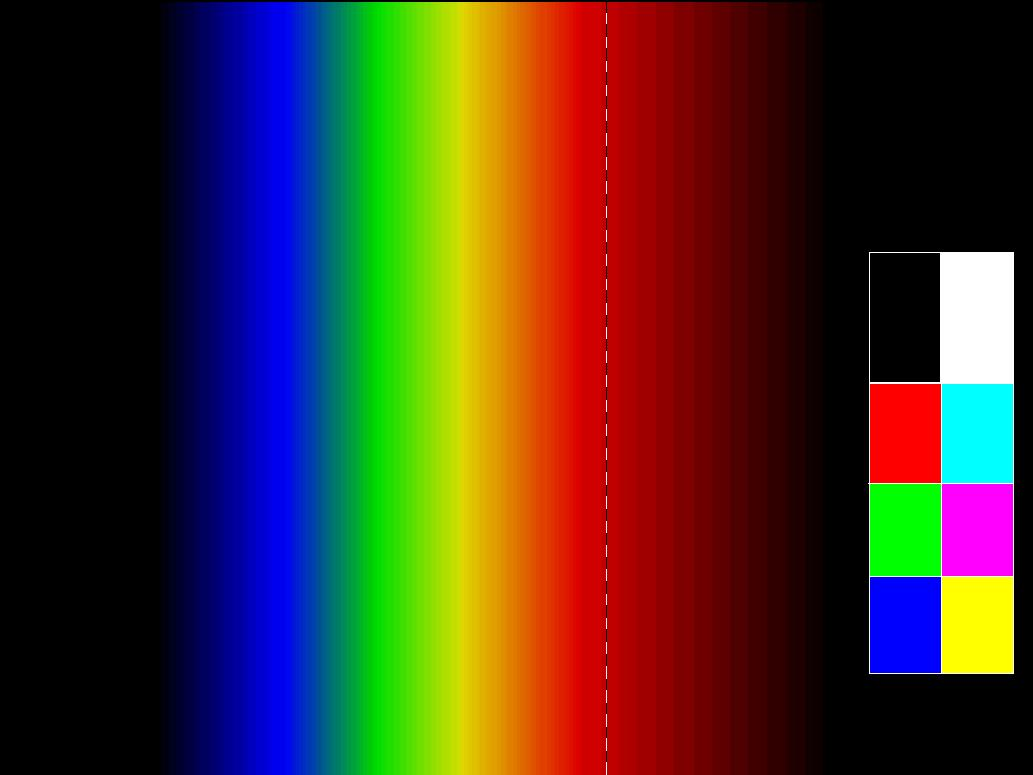
\includegraphics[width=\textwidth]{Graphics/opencvEtalon.jpg}
					        \caption{Spectre de la lumière visible \textit{\textbf{(source : http://physique-eea.ujf-grenoble.fr/)}}}
					    \end{subfigure}\\

					    \begin{subfigure}[h]{0.3\textwidth}
					        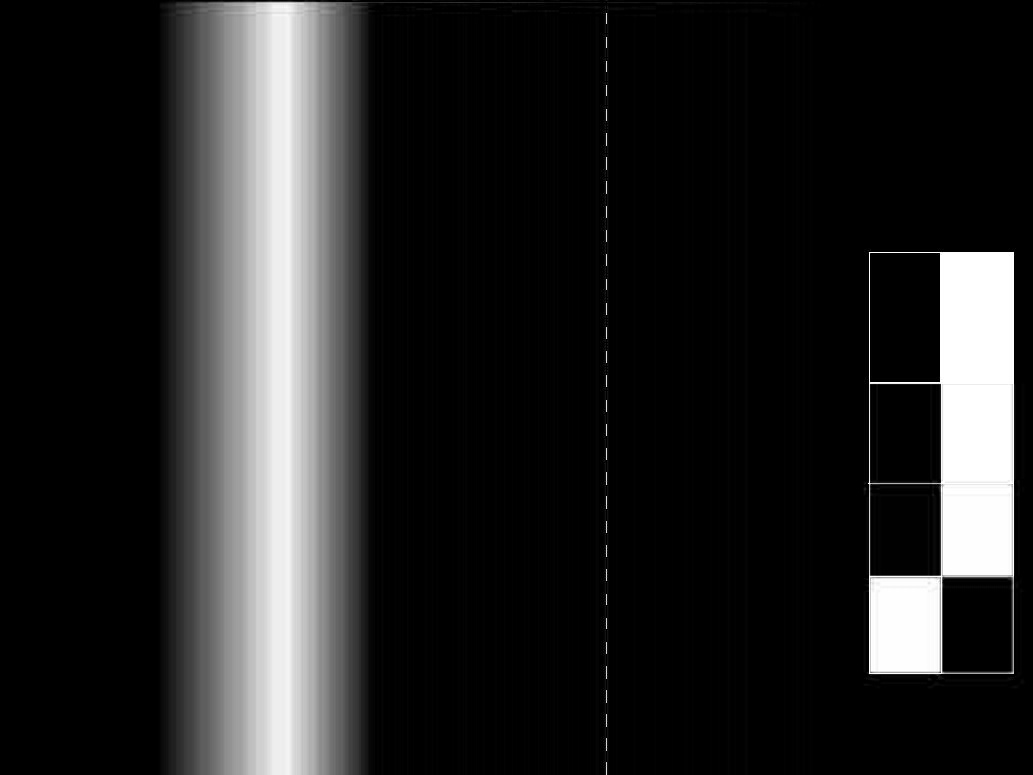
\includegraphics[width=\textwidth]{Graphics/opencvB.jpg}
					        \caption{Filtre bleu}
					    \end{subfigure}
					    ~ %add desired spacing between images, e. g. ~, \quad, \qquad, \hfill etc. 
					      %(or a blank line to force the subfigure onto a new line)
					    \begin{subfigure}[h]{0.3\textwidth}
					        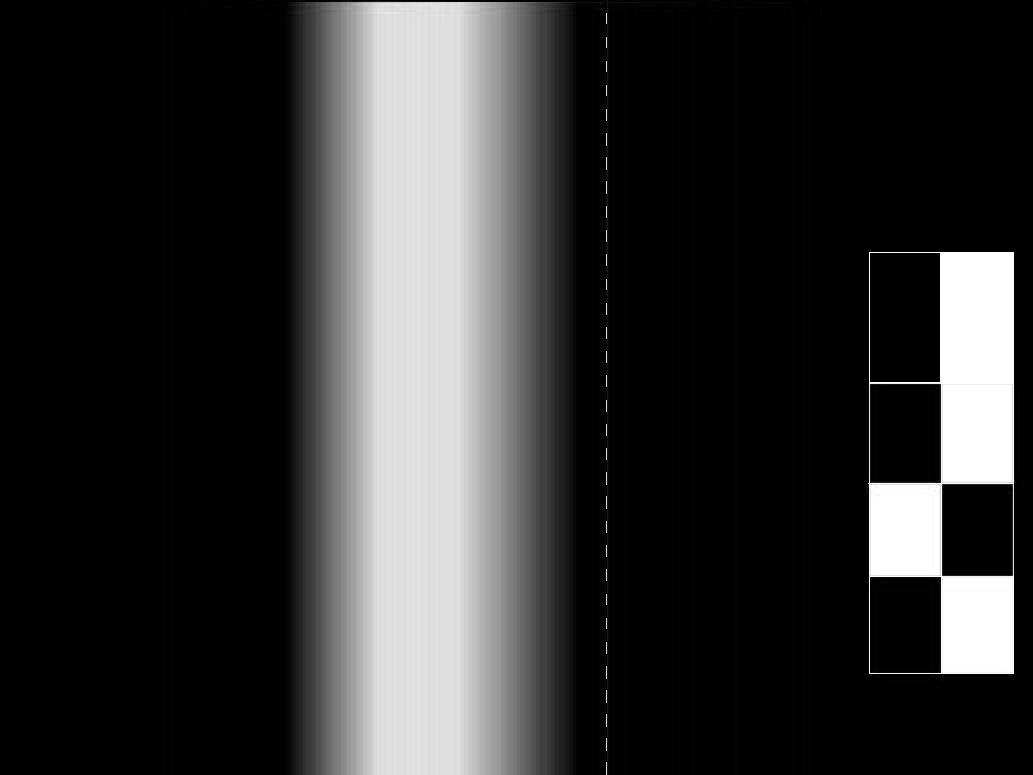
\includegraphics[width=\textwidth]{Graphics/opencvG.jpg}
					        \caption{Filtre vert}
					    \end{subfigure}
					    ~ %add desired spacing between images, e. g. ~, \quad, \qquad, \hfill etc. 
					    %(or a blank line to force the subfigure onto a new line)
					    \begin{subfigure}[h]{0.3\textwidth}
					        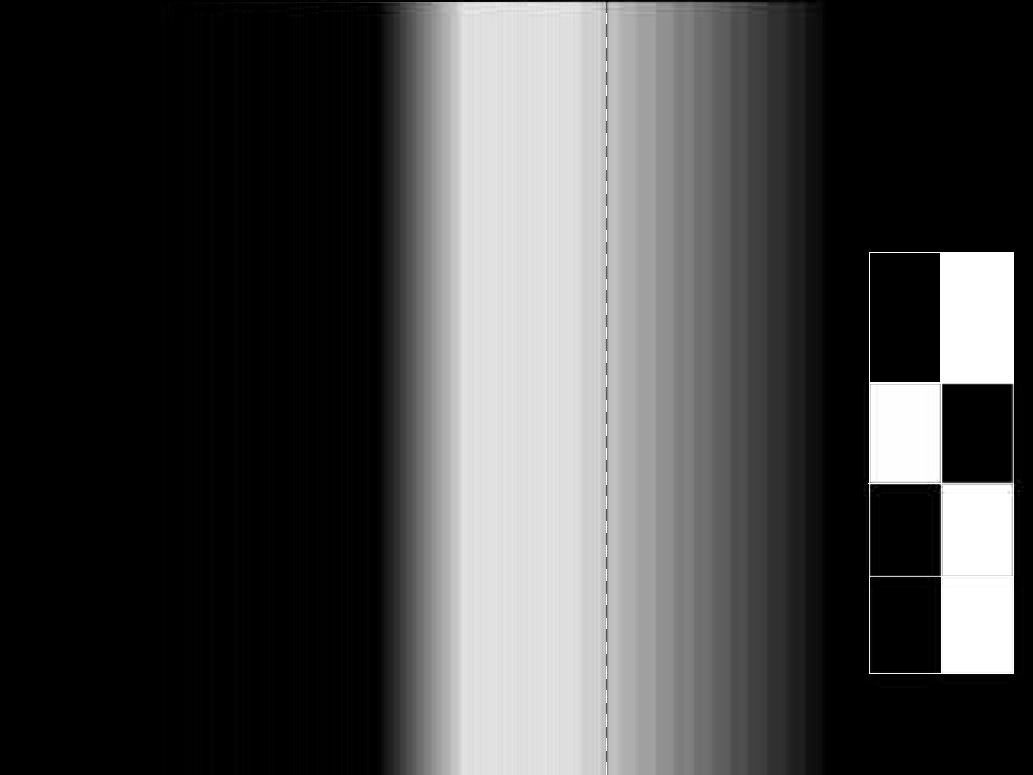
\includegraphics[width=\textwidth]{Graphics/opencvR.jpg}
					        \caption{Filtre rouge}
					    \end{subfigure}

					    \caption{Spectre (a), selon différents filtres (b),(c) et (d).}
					\end{figure}

					Pour des soucis d'optimisations et de résultats, nous n'utiliserons pas le système Rouge-Vert-Bleu classique, mais plutôt le système \label{HSV}\nomenclature{HSV}{Hue Saturation Value, ou Teinte Saturation Valeur} :

					\begin{figure}[H]
						\centering
						\begin{subfigure}[h]{0.35\textwidth}
					        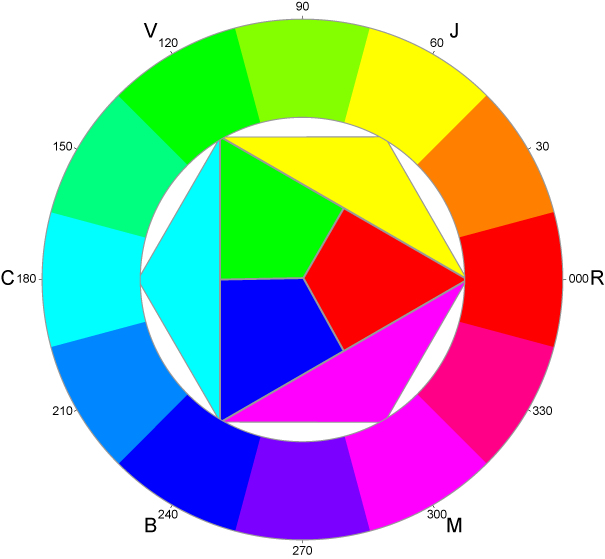
\includegraphics[width=\textwidth]{Graphics/RVB.png}
					        \caption{Modèle RVB}
					    \end{subfigure}
					    ~
					    \begin{subfigure}[h]{0.35\textwidth}
					        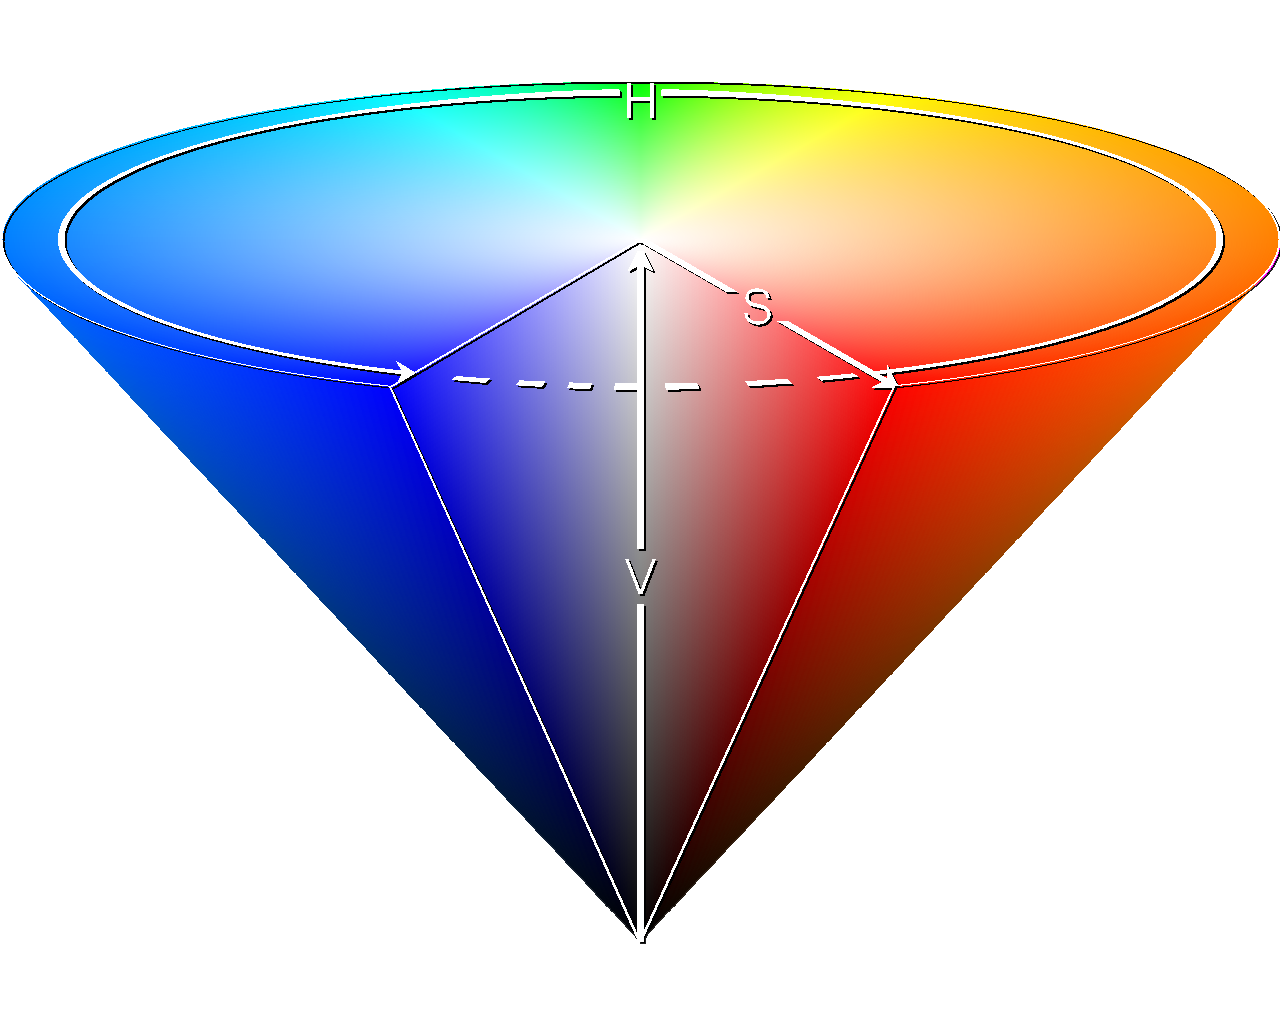
\includegraphics[width=\textwidth]{Graphics/HSV_cone.png}
					        \caption{Modèle HSV}
					    \end{subfigure}
					    \caption{Comparaison RVB / HSV}
					\end{figure}
					Grâce à ce système, il nous suffit de définir expérimentalement les bornes autour de nos 3 axes de couleurs afin de créer un \textit{masque}. Un masque est ici une image (une matrice, un tableau à deux dimensions); chaque case contenant "1" ou "0". Si "0", le pixel n'a pas passé le filtre : il ne nous intéresse pas. En revanche, si "1", ce pixel et ses environs sont potentiellement interessants et devront être analysés. Nous y reviendrons.
					La fonction \textit{inRange} est prévue à cet effet, et nous permet de réaliser un masque : 
					Nous déterminerons expérimentalement des bornes pour les variables Teinte ($H_{min}$ et $H_{max}$), Saturation ($S_{min}$ et $S_{max}$) et Valeur ($V_{min}$ et $V_{max}$). Soit un pixel $p$ positionné en $i$ avec pour composantes $H_{i,p}$,$S_{i,p}$,$V_{i,p}$, nous aurons la relation suivante :
					\\ 
					$D_i = H_{min} \leqslant H_{i,p} \leqslant H_{max} 	\land S_{min} \leqslant S_{i,p} \leqslant S_{max} \land V_{min} \leqslant V_{i,p} \leqslant V_{max}$ \cite{bib20}
					\\
					Avec $D_i$ valant VRAI ou FAUX. Si $D_i$ est FAUX, cela signifie qu'il n'y a aucune corrélation entre la couleur détectée et notre objet. En revanche, s'il est VRAI, alors notre objet existe PROBABLEMENT dans notre champs de vision. Nous définirons donc expérimentalement deux couples de triplets (correspondant aux bornes pour le feu vert et le feu rouge). De plus, en utilisant les fonctions d'érosion (\textit{erode}) et de dilatation (\textit{dilate}), nous suprimons les pixels parasites qui passeraient le premier filtre, gardant ainsi uniquement le feu.
					\\

					Une autre problématique est la distance à laquelle le robot doit s'arrêter. En effet, si le feu est rouge, il ne faut pas qu'il s'arrête juste à côté de celui-ci : il risquerait de ne pas le voir passer au vert et de rester bloqué. Compte tenu des vitesses engagées et de l'inertie des moteurs et du robot, nous négligerons la distance de freinage.
					Le schéma suivant résume la situation :
					\illu{distEval.pdf}{Schéma de principe de l'approche d'un feu}{0.35}
					Connaissant l'angle de vue de la caméra (58°)\cite{bib18}, et en utilisant des fonctions géométriques simples, nous pouvons déterminer rapidement la distance minimale au feu s'il faut s'arrêter : $d_{min} = 15 cm \times tan(\frac{58}{2}) = 8,3 cm$. En ajoutant une distance de sécurité puisque la distance de freinage est négligée, nous pouvons ainsi déterminer le moment à partir duquel le robot passera le feu quoi qu'il arrive. Cette distance est établie arbitrairement à 10 cm.\\

				\item \textbf{Présence et intentions des autres utilisateurs}

					Les feux sont les plus simples à gérer. En effet, il ne peut y avoir qu'une et une seule position pour un unique feu. Il suffit "juste" de détecter si oui ou non la couleur dans l'intervalle sélectionné existe. Détecter les intentions d'un autre robot est autrement plus difficile. En effet, compte tenu de la disposition des différents clignotants, nous voyons quoi qu'il arrive 3 des 4 clignotants du robot, s'il ne va pas dans le même sens que nous. 
					Un bon exemple d'un aperçu de la vue du robot est donné par la figure \ref{robotVueExemple}, page \pageref{robotVueExemple}.
					Après filtrage d'après la méthode indiquée ci-dessus, il faudra récupérer sur le masque de l'image obtenu les différentes tâches en utilisant une méthode itérative appelée MeanShift ("Déplacement de moyenne"). Le principe est simple : on choisit un point de coordonnées $(x_0,y_0)$. Autour de ce point, on définit une zone correspondant à la zone d'étude. On calcule donc la moyenne de chaque "1" du masque contenu dans la zone d'étude, ce qui nous donne un autre point de coordonnées $(x_1,y_1)$. l'opération est \textit{réitérée} autant de fois que nécessaire pour déterminer une LED. Le même procédé est appliqué une seconde fois. L'algorithme veut qu'un point "cherchant une LED" ne rentre pas dans la zone d'étude d'un autre point ayant déjà localisé une LED, afin de ne pas créer de doublon pouvant fausser les résultats. Si cette deuxième recherche de led est infructeuse, cela signifie que l'on se situe dans un des deux cas suivants :

					\begin{figure}[H]
						\centering
						\begin{subfigure}[h]{0.2\textwidth}
					        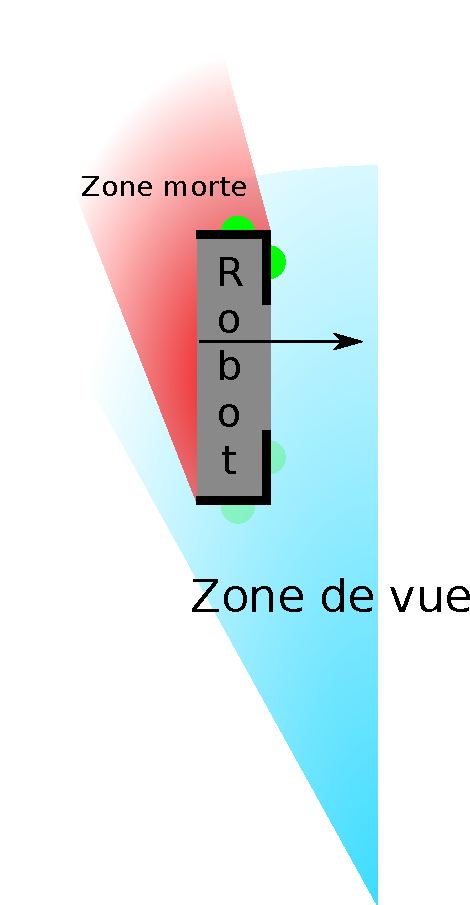
\includegraphics[width=\textwidth]{Graphics/casClignotants_DG.pdf}
					        \caption{Robot à gauche tournant à gauche}
					    \end{subfigure}
					    ~
						\begin{subfigure}[h]{0.35\textwidth}
					        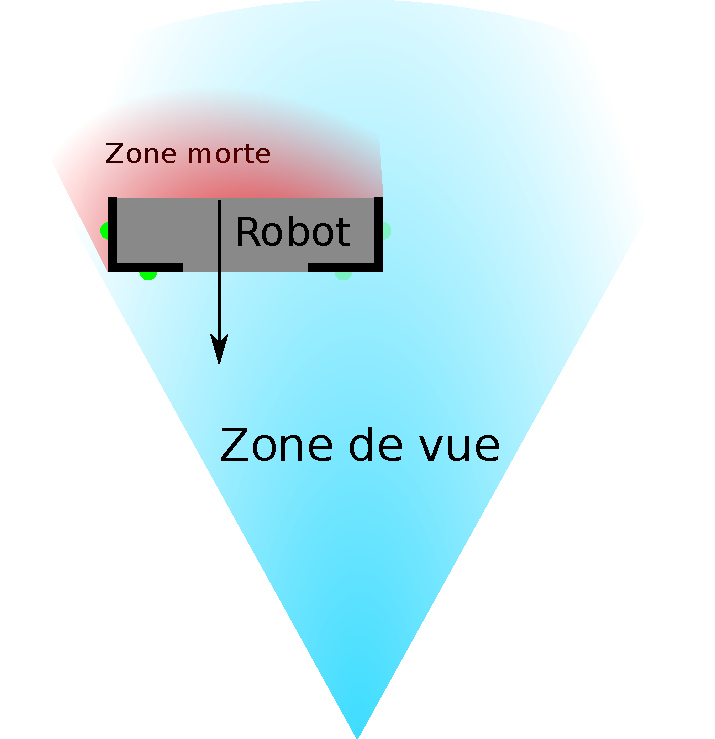
\includegraphics[width=\textwidth]{Graphics/casClignotants_AD.pdf}
					        \caption{Robot devant tournant à droite}
					    \end{subfigure}
					    ~
					    \begin{subfigure}[h]{0.2\textwidth}
					        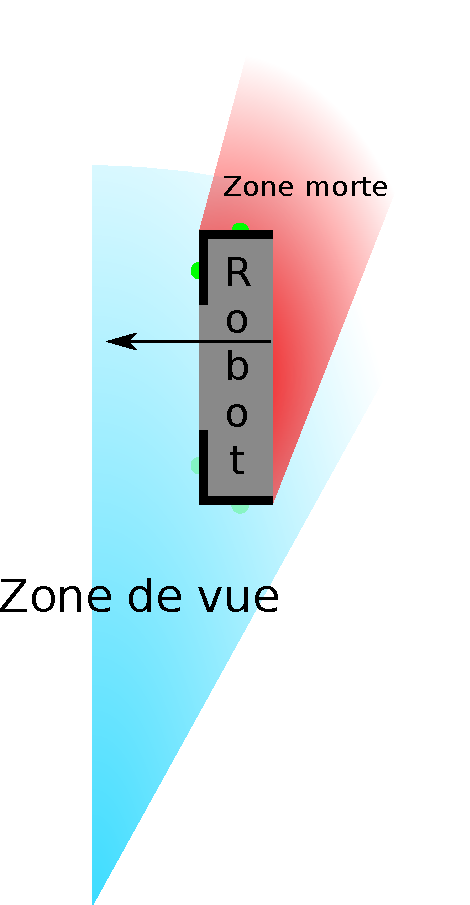
\includegraphics[width=\textwidth]{Graphics/casClignotants_GD.pdf}
					        \caption{Robot à droite tournant à droite}
					    \end{subfigure}
					    \caption{Cas d'une seule LED détectée}
					\end{figure}
					Si une situation comme cela apparait, on repère la position abolue de la LED. Si celle-ci se trouve sur la moitié droite du masque, cela signifie que l'on se situe dans le cas (c). Si la LED se situe sur le bord gauche, deux possibilités s'offrent à nous : soit on se trouve dans la situation (b), auquel cas on se situera au carrefour. Si notre feu est vert et que l'on décide de tourner à gauche également, il faudra combiner ces données au sonar. Si on décide d'aller tout droit ou à droite, on pourra traverser le carrefour sans soucis. En revanche, si on se trouve dans la situation (a), on a à nouveau deux possibilités : soit on se situe au carrefour central auquel cas un des deux robot sera arrété à cause du feu, donc aucun danger, soit on se trouve à une intersection : la règle de la priorité à droite d'applique, nous pouvons avancer sans être inquiétés.
					\\
					Voici les trois autres cas restants :
					\begin{figure}[H]
						\centering
						\begin{subfigure}[h]{0.2\textwidth}
					        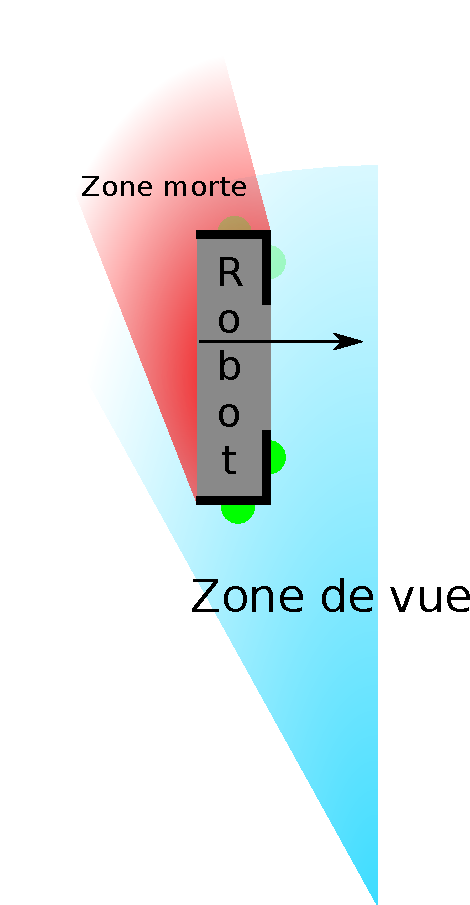
\includegraphics[width=\textwidth]{Graphics/casClignotants_DD.pdf}
					        \caption{Robot devant tournant à gauche}
					    \end{subfigure}
					    ~
						\begin{subfigure}[h]{0.35\textwidth}
					        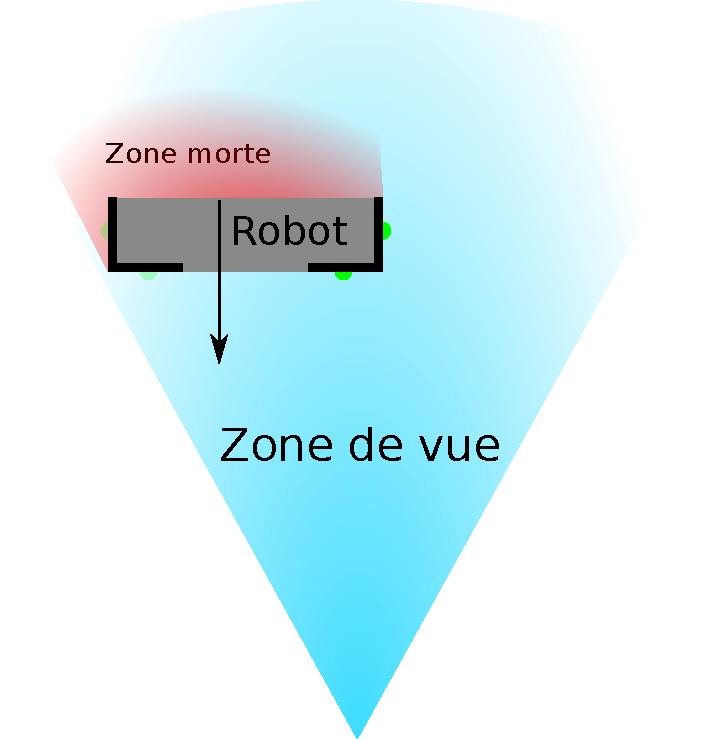
\includegraphics[width=\textwidth]{Graphics/casClignotants_AG.pdf}
					        \caption{Robot devant tournant à gauche}
					    \end{subfigure}
					    ~
					    \begin{subfigure}[h]{0.2\textwidth}
					        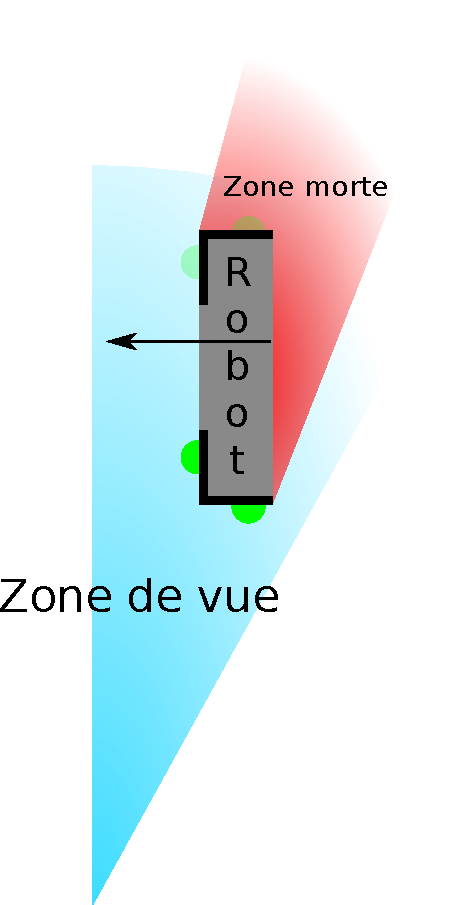
\includegraphics[width=\textwidth]{Graphics/casClignotants_GG.pdf}
					        \caption{Robot à droite tournant à gauche}
					    \end{subfigure}
					    \caption{Cas de deux LEDs détectées}
					\end{figure}

					Une fois encore, on réalise un masque et on repère la position des 2 LEDs. Cette fois, on "découpe" le masque en trois verticalement : si les LEDs sont dans le tier de gauche (a), l'agent est à gauche et désire tourner à droite. Si les LEDs sont dans le tier de droite (c), le robot, situé à droite, souhaitera tourner à gauche, et donc croiser notre trajectoire. Il s'agira là de faire respecter la règle de la priorité à droite. Enfin, si celles-ci sont dans le tier du milieu (b), cela signifie que le robot est en face et désire tourner à gauche, et croiser notre trajectoire.
			\end{itemize}

\newpage
\section{Intégration}

	\subsection{Circuit}

	\subsubsection{Intégration Matérielle}

		\paragraph{Circuit en lui-même}
			Notre circuit sera donc bien composé de deux parties, chacune constituée d'un panneau de médium monté sur un cadre en tasseaux.
			D'autres problématiques ont fait leur apparition en cours d'étude du projet et c'est ainsi que l'on intègrera des perçages pour la fixation des feux et le passage des fils, mais surtout pour l'intégration des fameux "caches" permettant d'isoler visuellement les "rues".\\

			Les panneaux seront peints en noir et recouverts de scotch d'électricien blanc représentant les lignes. Nous obtenons ainsi un rapport de contraste idéal (noir mat du bois et blanc brillant du ruban adhésif). Le plan à l'échelle de la piste est le suivant :
			\illu{CIRCUIT.pdf}{Plan à l'échelle de la piste}{0.065}

			\vspace{15pt}

			Y apparaissent les lignes, code-barres et caches (en gris plein) évoqués dans le dossier. Les rayons de courbure sont de 75mm, et l'espacement entre les voies et divers obstacles de 220mm.\\

			Un plan contenant toutes les côtes sera produit et pourra être "recopié" à l'aide de simple matériel scolaire (compas, règle, équerre) sur les panneaux avant d'être recouvert par le ruban adhésif.\\

			Les capteurs ILS seront fixés aux panneaux.\\
			On prévoiera des vis "dépassant" aux emplacements appropriés afin de pouvoir y "emboiter" les feux.\\

			Le câblage des capteurs et des feux sera solidaire de chaque partie, et passera par des trous prévus à cet effet dans les tasseaux pour converger en un "faisceau" terminé par un connecteur pour chacune des deux parties. Un connecteur sera présent du côté de chaque feu avec suffisemment de longueur de câble pour pouvoir facilement procéder à l'installation desdits feux.

			Voici à quoi ressemblerait le circuit (les petits éléments ne sont pas visibles):
			\illu{CIRCUIT2.png}{Modélisation 3D du circuit}{0.12}

		\paragraph{Carte électronique}

			La carte aura pour but de servir d’interface entre la carte FPGA et les composants électroniques du circuit (LEDs des feux bicolores et capteurs ILS).\\
			Comme évoqué précédemment, deux faisceaux de câbles terminés par des connecteurs arriveront sur cette carte (un pour chaque moitié de circuit). Ces faisceaux seront constitués de dix fils correspondant à :

			\begin{itemize}
				\item Masse feu 1
				\item Masse feu 2
				\item LED verte feu 1
				\item LED rouge feu 1
				\item LED verte feu 2
				\item LED rouge feu 2
				\item Retour ILS 1
				\item Retour ILS 2
				\item Alimentation ILS 1
				\item Alimentation ILS 2
			\end{itemize}

			Les cartes FPGA Basys 2 utilisées à l’IPSA disposent de quatre ports d’extensions dits « pmod » \cite{bib22}. Ces ports ont un format on ne peu plus standard : connecteurs femelles espacés d’un dizième de pouce.\\
			Chaque connecteur fournit 6 contacts :\\
			\begin{itemize}
				\item Une sortie 3,3V
				\item Une Masse
				\item 4 ports d’entrée/sorties directement mapés sur le FPGA.
			\end{itemize}

			\illu{pmod.png}{Illustration d'un port "pmod" \textbf{\textit{(source : Digilent)}}}{0.4}

			Les LEDs seront commandées par des ports du FPGA configurés en sortie.\\
			Pour ne pas tirer trop de courant sur ces ports (qui ne sont pas fait pour : il sont conçus pour produire des signaux et non des alimentations) et pouvoir fonctionner aussi bien en logique TTL que CMOS, nous passerons par un circuit intégré de la famille 74HC (\textbf{attention à bien différencier la série 74HC de la série 74HCT que nous serons également amenés à utiliser : elles n'ont pas les mêmes tensions de référence !}). 
			Ces portes logiques reposent sur la technologie « collecteur ouvert » et peuvent donc être utilisés comme des transistors de faible puissance. Les entrées logiques correspondent aux bases, les sorties aux émetteurs et l’alimentation du composant (Vcc) aux collecteurs.\\

			La datasheet \cite{bib24} nous apprend qu’ils peuvent fournir jusqu’à 50mA en sortie sur l’ensemble des sorties. En répartissant 4 LEDs par circuit logique et en utilisant ces dernières à 10mA (largement suffisant pour des LEDs  haute luminosité), nous restons en dessous de cette limite même lorsque les 4 LEDs sont allumées simultanément (ce qui en théorie ne devrait pas être le cas).
			Nous utiliserons le 74HC04 qui est un sextuple inverseur (seul 4 éléments seront utilisés). Ainsi, en plaçant un « 1 » (3.3V ou 5V : les deux fonctionnent puisque le composant reconnaît une valeur haute à partir de 2,3V) en entrée, nous obtenons 0V en sortie. En y plaçant un « 0 » (0V), nous obtenons un 3.3V jusqu 20mA par sortie pour un total de 50mA maximum ! Le tout sans jamais prélever plus d’un milliampère en entrée (et donc en sortie du FPGA).\\

			Les sorties du 74HC04 pourront être directement connecés aux anodes des LEDs via une résistance appropriée (150$\Omega$ pour une LED rouge à 1,8V de chute et 100$\Omega$ pour une LED verte à 2,3V de chute).\\


			L’acquisition des états des capteurs ILS est encore plus simple : les ILS étant de simples interrupteurs, on placera l’une de leurs bornes à la masse et on connectera l’autre à une entrée du FPGA en intercalant une résistance de pull-up placée à 3.3V.\\
			Ainsi, la carte FPGA verra un signal stable au niveau haut qui ne passera au niveau bas que lorsqu’un aimant excite le capteur.\\

			Nous pourrions simplifier et « sécuriser » le circuit en intégrant une partie de la logique de fonctionnement de manière électronique (penser le circuit pour que deux LEDs du même feu ne puissent-être allumées simultanément, par exemple), mais ceci irait à l’encontre de la vocation pédagogique du système et limiterait sa capacité d’évolution.\\

			Nous utiliserons de simple connecteurs sécables standard pour connecter le circuit à la carte Basys 2. Ainsi, on pourra directement « enficher » les deux cartes. Mais si l’IPSA venait à acheter de nouvelles cartes FPGA, l’utilisation de simples câbles « strips » permettra de se dispenser de refaire la carte.\\

			\illu{secable.png}{Illustration d'un connecteur sécable 0.1'' standard \textbf{\textit{(source : Gotronic)}}}{0.5}

			Nous aurions voulu mettre en place un système permettant de s’assurer que la carte ne peut être branchée que « dans le bon sens » (avec des connecteurs asymétriques par exemple) mais nous dépendons des connecteurs de la Basys 2 et ne pouvons implémenter cette sécurité. Il faudra donc être extrêmement attentifs à l’utilisation qui sera faite des cartes pour ne craindre aucun dommage (un analyse rapide des schémas nous montre cependant que peu de mal peut être infligé par un mauvais branchement). Surtout, la carte Basys2 est équipée sur ses ports pmod de diodes et résistances de protection \cite{bib23}.

	\subsubsection{Intégration Logicielle}

		Le cas du feu de circulation s'adaptant au trafic est l'exemple type de la logique dite de "l'automate fini". La littérature ne manque pas à ce sujet et nous avons même eu l'occasion de l'étudier au cours de notre cursus.\\

		La logique VHDL \nomenclature{VHDL}{VHSIC1 Hardware Description Language : langage destiné à la programmation de cartes FPGA.} est particulièrement adaptée à ce type de problématique et offre la possibilité de coder un certain nombre d'états et de définir les conditions et modalités de changement d'état.\\

		Dans notre cas, nous compterions trois états:
		\begin{itemize}
			\item \textbf{Etat 0} : Tous les feux au rouge.
			\item \textbf{Etat 1} : Couple de feux A au rouge et couple B au vert.
			\item \textbf{Etat 2} : Couple de feux B au rouge et couple A au vert.
		\end{itemize}

		\vspace {12pt}
		Une succession classique d'états serait 0->1->0->2->0->...\\
		Pour simplifier l'organisation du programme, nous pourrions créer un état intermédiaire entre 1 et 2, identique à l'état 0.\\

		Un diviseur d'horloge permettrait de générer des événements à intervalles réguliers afin de cadencer le changements d'états.\\
		Les capteurs eux-mêmes pourraient générer un événements (sur un front montant de l'entrée logique à laquelle ils sont branchés par exemple) qui, si un certain nombre de conditions sont réunies, anticiperaient le changement d'état (si une voiture se présente à un feu rouge et qu'aucune ne "profite" des feux verts, alors il est plus logique d'inverser cet état).

\subsection{Robot}

	\subsubsection{Intégration Matérielle}

		\paragraph{Ensembles propulsifs}

			Les deux "ensembles de propulsion" seront placés à l'arrière du robot. Une simple bille multidirectionnelle sera placée l'avant pour assurer la stabilité du robot.\\

			Le choix de notre motoréducteur fut basé sur un ensemble de critères :
			\begin{itemize}
				\item Le motoréducteur doit nous permettre d’atteindre une vitesse de pointe minimum de 15 cm/s (environ 70 tours par minute pour une roue de diamètre 4cm).
				\item Le motoréducteur devrait bénéficier d'un couple "confortable" pour les manoeuvres du robot.
				\item Le moteur ne devra pas être surdimensionné de manière à maîtriser la consommation d’énergie.
				\item On se munira du moteur le moins cher répondant aux critères précédents.
				\item Nous désirions aussi dans la mesure du possible trouver un moteur possédant un encodeur intégré, cependant ce critère ne correspond pas à un critère d’arrêt.
			\end{itemize}

			Nous avons estimé le couple minimum nécessaire à 0,01Nm par moteur (en effectuant le calcul pour différentes masses et inclinaisons de la piste).\\

			Il a ensuite fallu composer avec l'offre limitée présente sur le marché "semi-amateurs".\\

			Nous avons finalement sélectionné le motoréducteur "High-Power" de Pololu dans sa version proposant un taux de réduction de 298 pour 1.
			Ce moteur propose les caractéristiques suivantes :\cite{bib8} \\

			\begin{itemize}
				\item Couple de blocage de 0,5Nm
				\item Vitesse à vide sous 6V de 100 tours par minute
				\item Courant à couple maximum de 1.6A (soit 400mA maximum en utilisation normale)
			\end{itemize}


			Ce motoréducteur est associable avec une roue et un encodeur du même constructeur qui forment un ensemble fonctionnel et simple à implémenter. Nous y associerons un support PVC adapté pour la fixation.\\
			Notons qu'un seul des deux moteurs sera équipé d'un encodeur, deux étant superflus et évidemment plus chers.

			Le motoréducteur est équipé de deux fils d'alimentation. Nous les connecterons à la carte-mère au travers d'un bornier. Un double pont en H intégré L293D (comprenant les diodes de roue libre \cite{bib17}) permettra de faire le lien entre le signal PWM généré par le BBG (3.3V limité à une vingtaine de milliampères) et le moteur (que l'on alimentera directement sur la batterie, le signal PWM étant donc adapté sur une base 7.2V). Trois sorties seront donc utilisées sur le BBG pour chacun des deux moteurs : une PWM pour gérer la puissance transmise au moteur, et deux digitales pour le sens de rotation. Ces signaux (de 3.3V) pourront-être directement transmis au double pont en H (le L293D ayant une tension "niveau haut" de 2,3V \cite{bib17}). Nous compterons deux sources d'alimentation pour le pont en H : une alimentation de 5V pour le circuit logique et une alimentation directe sur la batterie (on pensera à intégrer deux condensateurs pour filtrer le bruit dû aux moteurs). Les signaux logiques viendront directement du BBG.\\

			Pour plus de détail, voir \ref{carteMere} (page \pageref{carteMere}).\\

			L'encodeur peut, d'après sa fiche technique \cite{bib9} fonctionner en 3.3V. Cependant, la diode émettrice IR perdra alors de son intensité. Nous procéderons donc à une expérience pour définir si ce fonctionnement en "sous régime" de la diode est satisfaisant. Dans le cas contraire, nous alimenterons l'encodeur en 5V et procéderons à une division de tension sur le signal de sortie avant de le transmettre au BBG, pour ne pas endommager ce dernier. Notons qu'un seul des deux "canaux" de l'encodeur nécessitera d'être connecté au BBG étant donné notre besoin de précision. Ainsi, la carte- mère devra comprendre un connecteur trois contacts dédié à l'encodeur : deux contacts serviront simplement à l'alimentation, et le troisième (le signal) sera connecté à l'une des entrées du BBG permettant l'utilisation du module eQEP (voir \ref{eQEP}).

		\paragraph{Carte Réflecteurs Optiques}\label{integrationReflecteurs}

			Rappelons que nous utiliserons les entrées analogiques du BBG pour effectuer l'acquisition des données du capteur, et que ces dernières sont limitées à 1.8V (voir \ref{solutionSuiviLigne}, page \pageref{solutionSuiviLigne}).

			La datasheet du TCRT5000 \cite{bib7} nous apprend que la LED émettrice possède une tension directe de 1.25V et n'accepte que jusqu'à 60mA.
			Afin de ne pas surcharger la sortie à 1.8V fournie par le BBG (qui ne fournit pas plus de 50mA), nous alimenterons les LEDs en 5V via une résistance de 120$\Omega$, faisant ainsi traverser la LED par $\frac{5-1.25}{120}=31mA$, ce qui est idéal (intensité IR\nomenclature{IR}{Infra-Rouge} suffisamment élevée sans risquer "d'éblouir" les autres capteurs ou de griller la LED).\\

			On connectera le collecteur du phototransistor à la ligne 1.8V au travers d'une résistance de pull-up de 2.7k$\Omega$, la valeur la plus élevée de résistance nous permettant d'assurer un courant de collecteur de 5mA (comme recommandé dans la datasheet). Nous choisissons la valeur la plus élevée afin de limiter la consommation en courant, mais surtout d'augmenter la sensibilité du capteur (il sera ainsi plus facile au phototransistor de "tirer" la tension vers le bas).\\

			Nous avons donc le schéma de principe suivant :
			\illu{reflecteur.pdf}{Schéma de principe d'un réflecteur optique}{2}

			Ce schéma sera reproduit sept fois sur une carte dédiée, qui sera placée à l'avant du robot, parfaitement centrée et placée quelques millimètres au dessus de la piste (la datasheet nous apprend que la distance de fonctionnement idéale entre le capteur et le support est de 2.5 mm, avec un domaine de fonctionnement allant de 0.2 à 12mm).\\
			
			Sachant que la ligne au sol aura une épaisseur de 15mm, nous placerons les trois capteurs centraux de manière à ce que, lorsque le capteur central est placé au milieu de la ligne, il ne manque que 2 à 3mm aux deux autres pour y arriver . Les autres capteurs pourront avoir un écartement légèrement plus élevé :

			\illu{espacementReflecteurs.pdf}{Espacement des réflecteurs optiques}{0.8}

			Notons que la distance exacte entre les capteurs ne pourra être précisément définie que par l'expérience. En effet, nous n'avons aucune indication quant à la largeur du champ de détection du capteur.\\

			Nous connecterons la carte au moyen d'une nappe HE10 à 10 connecteurs.\\

			Le schéma électronique et les gerbers du circuit imprimés sont disponibles en annexe \ref{schemasCarteReflecteurs} (page \pageref{schemasCarteReflecteurs})

		\paragraph{Carte-Mère}\label{carteMere}

			La carte mère est le circuit imprimé permettant de relier véritablement les actions "logicielles" aux actions réelles. Les contraintes pour cette carte sont simples :
			\begin{itemize}
				\item De taille raisonnable, soit de la taille bu BBG
				\item Ne pas intégrer directement les composants ayant un impact sur l'environnement du robot (moteur, LEDs...), pour qu'en cas de défaillance, ainsi que toujours dans un esprit de modularité et d'amélioration continue, un élément soit interchangeable rapidement, par le biais de connecteurs standards.
				\item Facilement intégrable au BBG. L'idée est vraiment de réaliser un shield enfichable simplement.
			\end{itemize}
			

			Ce shield intègre une prise standard de type Barrel jack, et peut être alimenté par toute source de tension supérieure à 7V. 
			\illu{barrelJack.jpg}{Embase Barrel Jack \textbf{\textit{(source : Conrad.fr)}}}{0.1}
			En effet, les moteurs demandant plus de 5v, il fallait trouver un moyen d'abaisser cette tension. Nous avons donc opté pour un régulateur de tension 5v. L'inconvénient de ce type de composant réside dans le fait qu'ils nécessitent un différentiel minimal entre la tension d'entrée et la tension de sortie appellé "Chute de tension", ou "Dropout/Forward Voltage" en anglais. Le composant LM7805 nécessite d'être alimenté par au moins 7v \cite{bib21} pour pouvoir sortir une tension stabilisée à 5v.\\

			Nous avons également décidé d'intégré un interrupteur à levier de type On/Off, afin d'économiser la batterie lorsque les moteurs ne sont pas nécessaires, et ainsi gagner en autonomie. Nous avons également inclu un bouton poussoir à impulsion (de type NO \nomenclature{NO}{Normally Open, Normalement ouvert}(On)/Off, selon les notations normalisées). Ce dernier démarrera la séquence de test, permettant ainsi de positionner le robot sur le circuit avant de commencer les tests.\\
			Les deux boutons sont accompagnés en dérivation de condensateurs. En effet, lors d'un changement d'état d'un interrupteur, le signal ne passe pas d'un état à un autre (de HAUT/HIGH à BAS/LOW ou inversement) immédiatement et parfaitement. Il y a une phase de transition qui, si elle n'est pas géré physiquement ou logiciellement, peut causer de graves problèmes, tel qu'un appui multiple, pouvant lancer plusieurs fois la séquence, entrainant des perturbations et pouvant potentiellement endommager le robot et/ou la carte. On parle de "debouncing", comme le présente la figure suivante :
			\begin{figure}[H]
				\centering
				\begin{subfigure}[h]{0.45\textwidth}
			        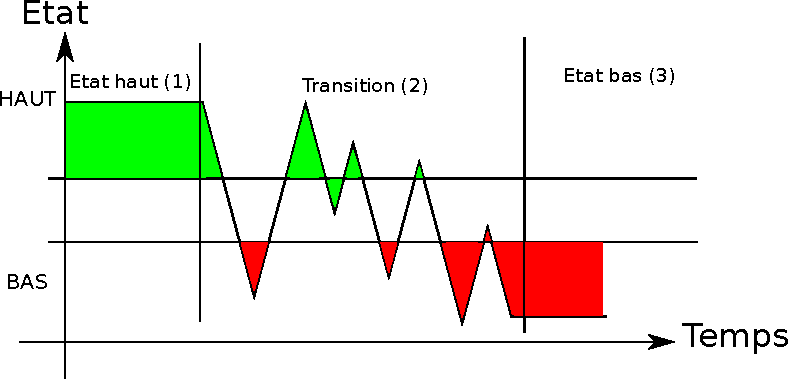
\includegraphics[width=\textwidth]{Graphics/btnNoDebounce.pdf}
			        \caption{Sans condensateur}
			    \end{subfigure}
			    ~
			    \begin{subfigure}[h]{0.45\textwidth}
			        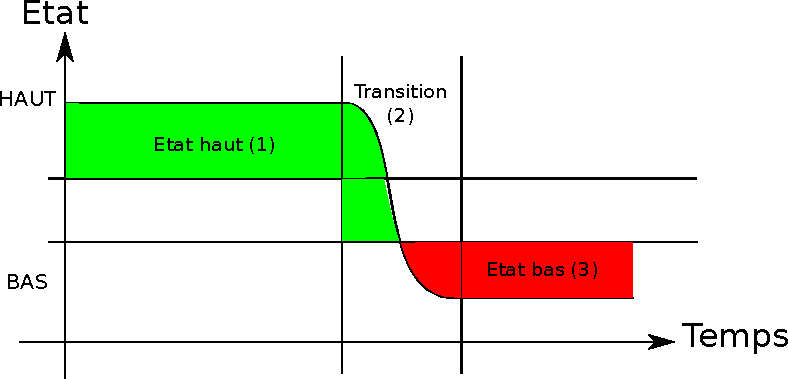
\includegraphics[width=\textwidth]{Graphics/btnDebounce.pdf}
			        \caption{Avec condensateur}
			    \end{subfigure}
			    \caption{Schéma de l'état d'un signal après l'ouverture d'un interrupteur}
			\end{figure}
			Grâce à ces schémas, on se rend rapidement compte de l'importance d'un simple composant passif. Dans le cas (a), le controlleur pourrait croire à de multiples pressions de l'interrupteur, pouvant engendrer des dommages au système mécanique, aussi bien qu'au système électrique. Dans le cas (b), le signal est continu et lissé. Il s'agit finalement d'un simple filtre passe-bas, puisqu'on a effacé toutes les hautes fréquences parasites.\\
			La carte mère est également pourvue d'un connecteur HE10-10, permettant une connexion simple et standard avec la carte réflecteurs. 
			\illu{he1010.jpg}{Connecteur femelle HE10-10 \textbf{\textit{(source : Conrad.fr)}}}{0.1}
			
			Le schéma de la Carte-mère a été réalisé grâce au logiciel Kicad, et est disponible en annexe, page \pageref{schemasCarteMere}.

		\paragraph{Structure du robot}

			L'intégration de tous les composants du robot passe forcément par un support, une structure d'ensemble.\\
			Nous avons choisi de réaliser cette structure sur une base de profilé aluminium de type "cornière égale" extrêmement simple à se procurer (dans toute enseigne de bricolage), peu chère, mais surtout très simple à usiner avec peu de matériel (l'aluminium étant très tendre, une simple visseuse suffit pour le perçage, une scie et une vis à métaux complétant l'outillage nécessaire).
			Un "cadre" en aluminium constituerai donc le châssis du robot. Ce cadre serait surmonté de quatre montants verticaux destinés à porter LEDs et caméra, et qui pourraient servir à fixer des "caches" pour fermer le robot (à la fois pour l'aspect esthétique et pour l'isolation lumineuse, afin de faciliter le travail de reconnaissance d'image). Un fond en médium ou en plexiglas abriterait le contrôleur et la batterie.\\

			L'idée maîtresse est de standardiser les matériaux et de penser au plus simple. Ainsi, nous essaierons tant que possible de tout faire avec un profilé aluminium unique (cornière égale de 30mm par 30mm), un seul type de vis et d'écrou (M3) et penserons notre assemblage de manière à être aisément réalisable, et ne présentant pas de risque de sur-contrainte.\\

			Le résultat vous est présenté à la section suivante : "Intégration globale, maquette numérique".

		\paragraph{Intégration globale, maquette numérique}

			Une maquette Catia nous a permis de définir le détail de la forme de la structure évoquée à la section précédente, mais également de prévoir l'intégration de tous les éléments.\\

			Tous les éléments de la maquettes ont été reproduits à partir des plans fournis par les constructeurs de composants sélectionnés. Ainsi, la maquette peut servir de plan d'usinage et de montage : aucune dimension n'est issue d'une quelconque approximation.

			\illu{ROBOT1.png}{Rendu de la maquette 3D du robot\label{robotVueExemple}}{0.4}
			\vspace{30pt}
			\illu{ROBOT2.png}{Rendu de la maquette 3D du robot}{0.4}

			\illu{ROBOT3.png}{Rendu de la maquette 3D du robot}{0.4}

			Le robot mesure 145mm de large (hors roues, 190 avec les roues), 200mm de long, et 150mm de haut.\\

			La maquette nous a permis d'évaluer le besoin en matériaux à :

			\begin{itemize}
				\item 1540mm de profilé aluminium.
				\item 4 vis M3 de 6mm de long.
				\item 24 vis M3 de 10mm de long (ou autant de vis auto-perçantes selon si l'on souhaite privilégier la facilité de fabrication ou la durée de vie).
				\item 10 vis M3 de 20mm de long.
				\item 34 écrous M3.
				\item 2 entretoises M3 de 15mm.
				\item 3 vis M2 de 10mm de long et autant d'écrous (pour le montage de la bille avant).
				\item une planche de medium de 3mm d'épaisseur en 140 par 200mm.
			\end{itemize}

	\subsubsection{Intégration Logicielle}\label{integrationLogicielle}

		L'intégration logicielle est sans aucun doute la partie la plus complexe de ce projet. Nous disposons d'un certain nombre d'entrées dont l'analyse simultanée permettra, au travers d'algorithmes relativement complexe, devra donner un ensemble de sorties cohérentes. Mais surtout, nous voulons que notre système soit modulaire, et que certaines parties de nos codes puissent être remplacés par d'autres, tout en assurant le fonctionnement des autres.\\

		Tout ceci ne pourra être effectué qu'au travers d'une architecture rigoureuse et largement pensée en amont (hors de question de se lancer dans le code comme on peut souvent le faire dans le cadre d'autres projets). Notons également que la construction d'une documentation et de codes clairement structurés et commentés sera également primordiale.\\

		Nous avons imaginé une structure en modules à quatre étages, au travers desquels l'information irait en descendant :

		\begin{itemize}
			\item \textbf{Les modules "Capteurs"} représenteraient le premier étage.\\
			Ces modules liraient directement la valeur des capteurs au travers des ports d'entrée physiques du contrôleur et produiraient une sortie adaptée.\\
			\textit{Par exemple, le module capteur" associé aux réflecteurs renverrait un vecteur de 7 bits correspondant à la présence ou non d'une ligne blanche sous chacun des capteurs : [1001001] correspondrait ainsi sans doute au passage d'un code barre. Plus compliqué, le module "capteur" associé à la caméra renverrait quatre matrices binaires 100x100 (une pour le vert, une pour le rouge, et une pour le jaune) dans lesquelles la présence d'un "1" indiquerait la détection d'une LED allumée aux cordonnées arrondies correspondantes.}
			\item \textbf{Les modules "Synthétiseur"} ne seraient pas liés à un capteur mais à une problématique. Ils pourront pour y répondre, analyser et synthétiser les données issues de plusieurs multiples modules capteurs.\\
			\textit{Ainsi, le synthétiseur lié à la problématique "lecture de codes barres" se renseignera auprès des modules capteurs "Réflecteurs optiques" et "Encodeur" afin de détecter la présence d'un code-barre et, le cas échéant, sa signification.}
			\item \textbf{Le module "Ordonnanceur"} serait a-priori unique. Il joue le rôle de chef d'orchestre et serait le seul module à intégrer la notion de temporalité (capacité de planification, et "mémoire" des événements récents). Ce serait également le seul module capable de faire "remonter de l'information" pour paramétrer le comportement des synthétiseurs.\\
			\textit{Par exemple, 25cm après la lecture d'un code-barre, l'ordonnanceur demanderait au synthétiseur dédié au suivi de ligne de ne plus se concentrer que sur une partie des réflecteurs optiques.}\\
			L'ordonnanceur fonctionnera forcément selon une logique séquentielle mais devra, pour être robuste et "clair", être décomposé en sous-modules (organe de décision, organe de planification, module dédié au gaz et module dédié à la direction, par exemple).
			\item \textbf{Les modules "Actionneurs"} recevraient des ordres (absolus ou relatifs) de la part de l'ordonnanceur et auraient pour rôle de les mettre en action au travers des sorties physiques du contrôleur.\\
			\textit{Concrètement, deux actionneurs géreront les sorties LEDs et les deux motoréducteurs. Un exemple "d'ordre absolu" pourrait-être "Vitesse = 0" tandis qu'un exemple d'ordre "relatif" serait "+5\% de rayon de virage".}
		\end{itemize}

		\vspace{15pt}

		Voici une simple illustration de la structure ici évoquée :
		\begin{figure}[H]
			\centering
			\begin{tikzpicture}[scale=0.7,transform shape]
 
  % Draw diagram elements
  \path \module {1}{Capteur 1};
  \path (p1.east)+(4.0,0.0)\module {2}{Capteur 2};
  \path (p2.east)+(4.0,0.0)\module {3}{Capteur 3};

  \path (p1.south)+(3,-2.0)\module {4}{Synthétiseur 1};
  \path (p2.south)+(3,-2.0)\module {5}{Synthétiseur 2};

  \path (p4.south)+(2.9,-2.0)\module {6}{Ordonnanceur};

  \path (p1.south)+(0.0,-7.0) \module {8}{Actionneur 1};
  \path (p2.south)+(0.0,-7.0) \module {9}{Actionneur 2};
  \path (p3.south)+(0.0,-7.0) \module {10}{Actionneur 3};

  \path [myArrow] (p1.south) -- + (0.0,-0.9) -- + (3.0,-0.9) -- node [above] {} (p4);
  \path [line] (p2.south) -- + (0.0,-0.9) -- + (-3.0,-0.9);

  \path [myArrow] (p2.south) -- + (0.0,-0.9) -- + (3.0,-0.9) -- node [above] {} (p5);
  \path [line] (p3.south) -- + (0.0,-0.9) -- + (-3.0,-0.9);

  \path [myArrow] (p4.south) -- + (0.0,-1.0) -- + (+2.9,-1.0) -- node [above] {} (p6);
  \path [line] (p5.south) -- + (0.0,-1.0) -- + (-3.2,-1.0);

  \path [myArrow] (p6.east) -- + (4.5,0) -- + (4.5,2.55) -- node [right] {} (p5);

  \path [myArrow] (p6.south) -- + (0.0,-0.5) -- + (-5.95,-0.5) -- node [above] {} (p8);
  \path [myArrow] (p6.south) -- node [above] {} (p9);
  \path [myArrow] (p6.south) -- + (0.0,-0.5) -- + (5.95,-0.5) -- node [above] {} (p10);

\end{tikzpicture}
			\vspace{10pt}
			\caption{Structure logicielle en "modules"}
		\end{figure}

		Tous ces modules constitueraient l'un des livrables du projet et seraient codés en python, en suivant une approche "objet". A sa réception, le robot devra pouvoir être mis sous tension et évoluer en autonomie. Mais le réel enjeu du projet sera de faire en sorte que ces modules soient parfaitement documentés et architecturés, de manière à ce qu'un utilisateur souhaitant, par exemple, développer son propre module de reconnaissance d'image en C++ puisse faire fonctionner ce dernier avec le reste de nos modules (pour ne pas avoir à se préoccuper d'une partie suivi de ligne qui ne l 'intéresse pas).\\
		Ceci sera rendu possible, notamment, par l'utilisation optionnelle (mais intégrée) de sockets locaux UDP pour communiquer entre les modules.\\

		Un programme principal aurait pour rôle de gérer l’exécution des différents modules, et de répartir intelligemment leur utilisation processeur. Ce programme, lui même codé en python, sera conçu pour fonctionner nativement avec l'ensemble de nos modules, mais sera également capable d’exécuter des modules tiers. Ce programme devra lui-même faire preuve d'une très grande rigueur. Son fonctionnement sera régi par la lecture d'un fichier de configuration à son initialisation. Ainsi, ce fichier de configuration pourra déterminer quels modules devront-être exécutés, et avec quel paramétrage.\\

		Un scenario possible serait :\\
		\textit{Exécuter tous les modules natifs sauf le module synthétiseur spécialisé en reconnaissance de feux qui sera remplacé par le programme "monProgramme.exe" placé à la racine. Le module capteur "sonar" devra communiquer sur le port 40052. Les autres modules seront chargés en configuration par défaut.}\\
		Ces instructions seraient définies dans le fichier de configuration, et leur exécution serait assurée par le programme principal. Évidemment, ceci ne pourra fonctionner que si l'utilisateur a très soigneusement suivi les recommandations de la documentation lui indiquant quel type de données doit fournir le module synthétiseur spécialisé en reconnaissance de feux.\\

		Encore une fois, rien n'obligera l'utilisateur à se servir de cette base logicielle. Il pourra très bien décider d'ignorer totalement le système en place et concevoir le sien. Le but de ce système est vraiment de permettre à un élève de se concentrer sur une problématique ciblée en voyant les autres traitées pour lui. Mais cela ne peut se faire que si son propre module n'empêche pas le fonctionnement des autres. Ceci ne peut être le cas que si son module est parfaitement additionnel (et fait donc un travail dont le résultat n'est requis par aucun autre module) ou si il est parfaitement compatible avec les autres (et transmet donc les données dans le même format et selon le même protocole que le module natif).\\

		Nous ne pouvons pas insister suffisemment sur le fait que ceci ne représente que l'approche théorique du problème. Si nous l'avons longuement pensé et réfléchi, ce travail n'est absolument pas suffisent pour donner lieu à une phase de développement : celle-ci devra être précédée d'une phase de préparation minutieuse, notemment en utilisant les outils de "Model Driven Engineering" (diagrames de classes, d'interaction...) afin de mettre en place un cadre de travail strict et rigoureux absolument nécéssaire à la réussite d'un projet de ce type.

\subsection{Synthèse}
	Pour mieux se représenter le système dans son ensemble, voici quelques mises en situation :\\
	\illu{miseEnSituation.png}{Mise en situation du robot sur le circuit}{0.5}
	\vspace{25pt}
	\illu{miseEnSituation1.png}{Mise en situation du robot sur le circuit}{0.5}
	\illu{miseEnSituation2.png}{Mise en situation du robot sur le circuit}{0.5}

\newpage
\section{Estimation du coût de mise en place et faisabilité}

	 Nous avons fait notre possible pour estimer les coûts liés à ce projet. Il s'agit évidemment d'un exercice complexe.
 Il est toujours plus simple d'évaluer le coût matériel que le coût humain. Ici, la main d'oeuvre est gratuite, mais il n'empêche qu'un planning réaliste serait un atout de taille pour mener ce projet à bien.

 \subsection{Fournitures}

 	Le descriptif technique détaillé élaboré au cours de ce dossier nous permet de dresser une liste précise et sans doute proche de l'exhaustivité du matériel nécessaire.\\

 	Celà nous a permis de définir les coûts suivants :
 	\begin{itemize}
 		\item Coût d'un robot : 270€ HT
 		\item Coût du circuit (hors impression 3D): 85€ HT
 		\item Coût du chargeur : 20€ HT
 		\item Coût des composants divers : 10€
 	\end{itemize}

 	\vspace{15pt}

 	Soit, pour un ensemble d'un circuit et deux robots, un total de \textbf{450€ HT} (525€ TTC).\\

 	Le détail des calcul est disponible en annexe \ref{devis} (page \pageref{devis}).



 	Nous avons sélectionné les principaux fournisseurs en fonction de la compatibilité de leur catalogue avec notre besoin.
 	Nous avons essayé de limiter le nombre de fournisseurs afin de simplifier la "logistique" et limiter les frais de port.\\

 	Heureusement, les fournisseurs sur Internet disposent aujourd'hui de très larges catalogues et nous n'avons pas été limités dans notre choix de composants.

 \subsection{Volume de travail}

 	Nous avons identifié plusieurs « work packages » :\\
 	\begin{itemize}
 		\item Fournitures
 		\item Réalisation des cartes
 		\item Assemblage du robot
 		\item Réalisation du circuit
 		\item Développement logiciel
 	\end{itemize}

 	\newpage

	Les tâches du projet ont été définies, estimées et réparties dans les « work packages » comme ceci :\\

	\illu{planning.pdf}{Estimation du planning}{0.87}

	\vspace{15pt}

	Ceci nous a permis d'établir les diagrammes de Gantt et de PERT, et donc d’en déduire un processus, une marche à suivre, pour la réalisation du projet.\\

	\illu{Gantt.png}{Diagramme de Gantt du projet (agrandissement disponible en annexe \ref{gantt})}{0.3}
	\vspace{15pt}
	Le chemin critique est représenté par les cases hachurées.\\

	Du diagramme de Gantt, nous avons pu déduire le diagramme PERT suivant:
	\illu{PERT1.png}{Diagramme PERT du projet (1/2) (agrandissement disponible en annexe \ref{PERT})}{0.6}
	\illu{PERT2.png}{Diagramme PERT du projet (2/2) (agrandissement disponible en annexe \ref{PERT})}{0.4}
	\vspace{15pt}
	Le chemin critique est représenté par les cellules en jaune.\\

	Ces diagrammes ont été réalisés en se basant sur l’hypothèse d'une disponibilité totale des ressources et de l'absence absolue d'imprévus. S'agissant évidemment d'une hypothèse parfaitement irréaliste, et malgré le "pessimisme" dont nous avons volontairement fait preuve pour estimer les volumes horaires, nous envisageons une majoration de la durée du projet et de la quantité de travail de l’ordre de 20\%.

\newpage
\section{Conclusion et aperçu des évolutions possibles}
	
	\input{chapitres/6_conclusion}

\setcounter{secnumdepth}{0}
\renewcommand{\thesubsection}{\Alph{subsection}}

\newpage
\sectionWoNum{Annexes}

	\subsection{Carte Réflecteurs Optiques}\label{schemasCarteReflecteurs}
	\subsubsection{Schéma électronique}

		\illu{ANNEXES/CARTE-REFLECTEURS_circuit.pdf}{Schéma électronique de la carte Réflecteurs Optiques}{1}

		\newpage
	\subsubsection{Gerbers}
		\illu{ANNEXES/CARTE-REFLECTEURS.pdf}{Gerbers de la carte Réflecteurs Optiques}{1}
	\subsection{Carte Mère}\label{schemasCarteMere}
	\subsubsection{Schéma électronique}

		\illu{ANNEXES/SCHEMA_CARTE_MERE_1.pdf}{Schéma du circuit de la carte mère}{1}
		\illu{ANNEXES/SCHEMA_CARTE_MERE_2.pdf}{Schéma du circuit de la carte mère}{1}


		\newpage
	\subsubsection{Gerbers}
		\illu{ANNEXES/CARTE_CARTE_MERE.pdf}{Gerbers de la carte mère}{1}

\setcounter{secnumdepth}{0}
\newpage
\section{Références}

	\subsection{Nomenclature} \label{nomenclature}
		\printnomenclature

	\newpage
	\nocite{bib11}
	\subsection{Bibliographie} \label{bibliographie}
		\begingroup
		\renewcommand{\section}[2]{}%
		\bibliography{includes/bibliography}{}
		\bibliographystyle{plain}
		\endgroup

	\newpage
	\subsection{Table des illustrations}
		\begingroup
		\renewcommand{\section}[2]{}%
		\listoffigures
		\endgroup
		
\newpage
\section{Résumé}
\end{document}